\documentclass[11pt]{article}
\usepackage{acl-hlt2011}
\usepackage{times}
\usepackage{latexsym}
\usepackage{amsmath}
\usepackage{multirow}
\usepackage{url}
\usepackage{graphicx}
%\DeclareMathOperator*{\argmax}{arg\,max}
%\setlength\titlebox{6.5cm}    % Expanding the titlebox
\setlength\titlebox{3.5cm}    % Expanding the titlebox

\newcommand{\mnote}[1]{\marginpar{\raggedleft\footnotesize\itshape#1}} 

%\title{Paraphrase Acquisition Combining Monolingual and Bilingual Information}
%\title{Re-ranking Paraphrases Extracted from Bilingual Parallel Corpora \\ Using Monolingual Distributional Similarity}
\title{Re-ranking Bilingually Extracted Paraphrases \\ Using Monolingual Distributional Similarity}

%\author{First Author \\
%  Affiliation / Address line 1 \\
%  Affiliation / Address line 2 \\
%  Affiliation / Address line 3 \\
%  {\tt email@domain} \\\And
%  Second Author \\
%  Affiliation / Address line 1 \\
%  Affiliation / Address line 2 \\
%  Affiliation / Address line 3 \\
%  {\tt email@domain} \\}

\date{}

\begin{document}
\maketitle
\begin{abstract}
This paper improves an existing bilingual paraphrase extraction technique using monolingual distributional similarity to re-rank candidate paraphrases.  Raw monolingual data  provides a complementary and orthogonal source of information that lessens the commonly observed errors in bilingual pivot-based methods. %We incorporate a newly developed locality sensitive hashing algorithm into the monolingual score calculation in order to facilitate a practical implementation of this method over large volumes of data. 
Our experiments reveal that monolingual scoring of bilingually extracted paraphrases has a significantly stronger correlation with human judgment for grammaticality than the probabilities assigned by the bilingual pivoting method does. The results also show that monolingual distribution similarity can serve as a decent threshold for high precision paraphrase selection.

%This shows promises in further improvement of paraphrase quality through merging of the variety of scores...@@

\end{abstract} 


\section{Introduction}
%\mnote{add back some details that were omitted due to acl short ppr constaint?}
%\mnote{note to self: revise according to notes from chris, ben and also in moleskin notebook}
Paraphrasing is the rewording of a phrase such that meaning is preserved. Data-driven paraphrase acquisition techniques can be categorized by the type of data that they use \cite{MadnaniDorr10}.  Monolingual paraphrasing techniques cluster phrases through statistical characteristics such as dependency path similarities or distributional co-occurrence information \cite{Lin01discoveryof,PascaDienes05}.   Bilingual paraphrasing techniques use parallel corpora extract potential paraphrases by grouping English phrases that share the same foreign translations \cite{BannardCallisonBurch05}.  Other efforts blur the lines between the two, applying techniques from statistical machine translation to monolingual data or extracting paraphrases from multiple English translations of the same foreign text \cite{Barzilay2001,PangEtAl03,QuirkDolanBrockett04}.

%Although the knowledge used by monolingual and bilingual paraphrasing techniques is largely orthogonal, only limited effort has been devoted to merging the two lines of work to develop new methodologies and applications. For instance, word-alignment from parallel monolingual data was used to train a phrasal ``translation" model \cite{QuirkDolanBrockett04}; paraphrases extracted from output of SMT trained on bilingual text are incorporated into query expansion for answer retrieval \cite{RiezlerEtAl07}.

%@@ include additional applications?@@
%Additional application of paraphrases in the domain of natural language processing includes text summarization (McKeown et al., 2002), headline or title generation (Dorr et al., 2003; Vandeghinste and Pan, 2004; Marsi et al., 2009,),  Recently paraphrase models has also been considered for sentence compression (?courtney's). An extensive survey of paraphrase methods is contained in \newcite{MadnaniDorr10}.

We exploit both methodologies, applying a monolingually-derived similarity metric to the output of a pivot-based bilingual paraphrase model.  
In this paper we investigate the strengths and weaknesses of scoring paraphrases using monolingual distributional similarity versus the bilingually calculated paraphrase probability.  We show that monolingual cosine similarity calculated on large volumes of texts ranks bilingually extracted paraphrases better than the paraphrase probability originally defined by \newcite{BannardCallisonBurch05}. While our current implementation shows improvement mainly in grammaticality, other contextual features are expected to enhance the meaning preservation of paraphrases. We also show that monolingual scores can provide a reasonable threshold for picking out high precision paraphrases. 

% Our work overlaps with their approach in the paraphrase generation with bilingual translation rules. However, instead of assigning paraphrase score based on phrase translation probabilities, we introduced a measure dependent on monolingual distributional similarity built upon large n-gram corpus. Locality sensitive hashing method of \newcite{Charikar02}, which has been recently extended to online signature generation by \newcite{VanDurmeLallACL10}, was implemented to enable faster computation by reducing the similarity feature space dimension with random projection. Descriptions on each stage of the process will be covered in the following sections, which are followed by examples and evaluation results.

%@@ previous work on paraphrasing reranking (monolingual and bilingual based?) @@


%\section{Related Work}
%@@ previous work on paraphrasing (monolingual and bilingual based); @@
%One example is the work on discovery of inference rule, analogous to paraphrasing, with parsed dependency trees  
%@@ Nitin Madnani's survey ppr on data driven paraphrase methods@@
%


%\section{Multilingual Paraphrase Extraction via Pivoting}
\section{Related Work}

\subsection{Paraphrase Extraction from Bitexts}

 \newcite{BannardCallisonBurch05} proposed identifying paraphrases by pivoting through phrases in a bilingual parallel corpora. 
Figure~\ref{paraphrase-illustration} illustrates their paraphrase extraction process. The \emph{target} phrase, e.g. {\it thrown into jail}, is found in a German-English parallel corpus.  The corresponding foreign phrase ({\it festgenommen}) is identified using word alignment and phrase extraction techniques from phrase-based statistical machine translation \cite{KoehnEtAl03}.  Other occurrences of the foreign phrase in the parallel corpus may align to another English phrases like {\it jailed}.  
%Following \newcite{BannardCallisonBurch05}, we treated any English phrases that share a common foreign phrase as potential paraphrases of each other.
%
As the original phrase occurs several times and aligns with many different foreign phrases, each of these may align to a variety of other English paraphrases.  Thus, {\it thrown into jail} not only paraphrases as {\it jailed}, but also as {\it arrested}, {\it detained}, {\it imprisoned}, {\it incarcerated}, {\it locked up}, and so on.
%{\it taken into custody}, and {\it thrown into prison} and others like {\it be thrown in prison}, {\it been thrown into jail}, {\it being arrested}, {\it in jail}, {\it in prison}, {\it put in prison for}, {\it were thrown into jail}, and {\it who are held in detention}. 
Bad paraphrases, such as
 {\it maltreated}, {\it thrown}, {\it cases}, {\it custody}, {\it arrest}, and {\it protection}, may also arise due to poor word alignment quality and other factors.

\newcite{BannardCallisonBurch05} defined a paraphrase probability to rank these paraphrase candidates,  as follows:
\begin{eqnarray} 
 \hat{e_2}	& = & \arg \max_{e_2 \neq e_1} p(e_2 | e_1)\label{paraphrase-prob}  
\end{eqnarray}
\begin{eqnarray} 
  p(e_2|e_1) &=& \sum_f p(e_2,f|e_1)\\
                  &=& \sum_f p(e_2|f,e_1) p(f|e_1) \\
                  &\approx& \sum_f p(e_2|f) p(f|e_1)
\label{paraphrase_prob_eqn}
\end{eqnarray}
where ${p(e_2|e_1)}$ is the paraphrase probability, and ${p(e|f)}$ and ${p(f|e)}$ are translation probabilities from a statistical translation model.  


\begin{figure}
\begin{center}
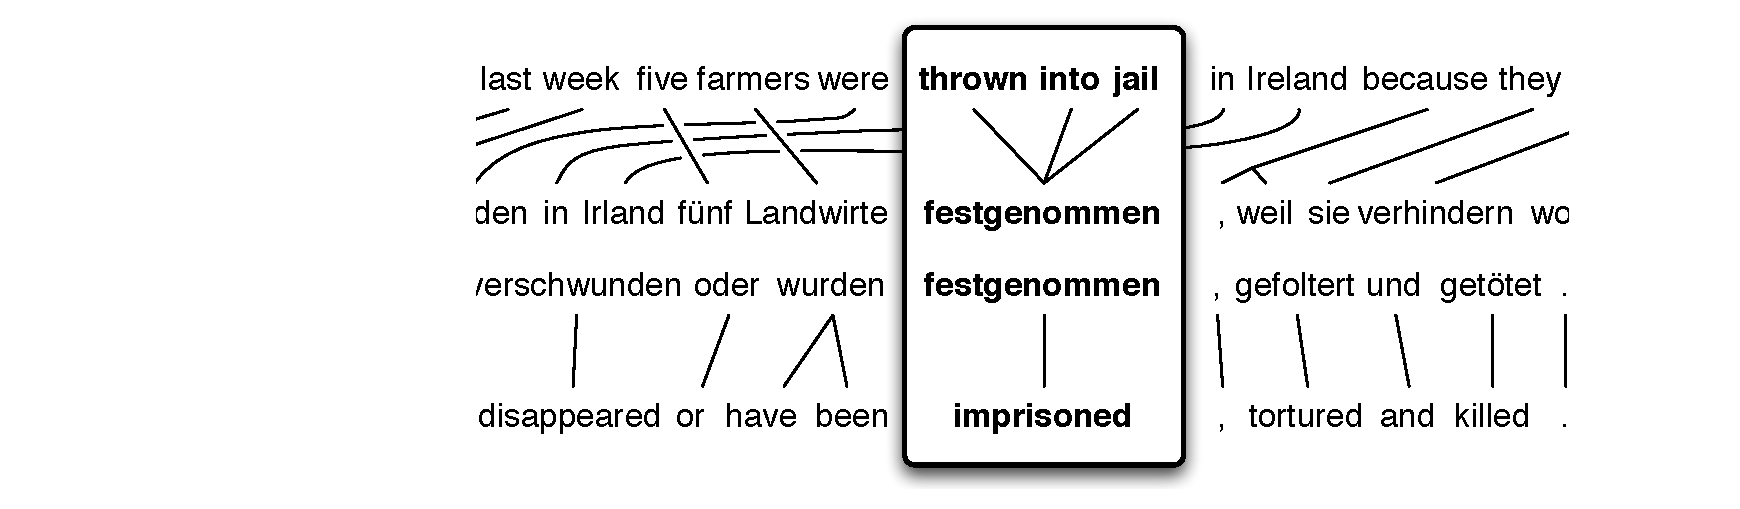
\includegraphics[width=\linewidth]{pivot-2}
\end{center}
\caption{\small Using a bilingual parallel corpus to extract paraphrases.}
\label{paraphrase-illustration}
\end{figure}

Anecdotally, this paraphrase probability sometimes seems unable to discriminate between good and bad paraphrases, so some researchers disregard it and treat the extracted paraphrases as an unsorted set \cite{Snover2010}.  \newcite{CallisonBurch08} attempts to improve the ranking by limiting paraphrases to be the same syntactic type.  

We attempt to re-rank the paraphrases using other information. This is similar to the efforts of \newcite{ZhaoEtAlACL08}, who made use of multiple resources %, namely the thesaurus, monolingual parallel corpus, monolingual comparable corpus, bilingual phrase table, dictionary definitions, clusters of similar user queries, and self paraphrase 
to derive feature functions and extract paraphrase tables. The paraphrase that maximizes a log-linear combination of various feature functions is then selected as the optimal paraphrase. Feature weights in the model are optimized by minimizing a {\it phrase substitution error rate}, a measure proposed by the authors, on a development set.
% using gradient descent. 

%In our work, we examine how bilingual and monolingual re-ranking metrics complement each other in order to effectively combine them.

\subsection{Monolingual Distributional Similarity}\label{section:monolingual-distributional-similarity}
%\section{Confidence Measure based on Monolingual Distributional Similarity}
%\section{Using Monolingual Resources}
\label{sect:mds}

Prior work has explored the acquisition of paraphrases using distributional
similarity computed from monolingual resources, such as in the DIRT results of
\newcite{Lin01discoveryof}. In these models, phrases are judged to be similar
based on the cosine distance of their associated context vectors. In some cases,
such as by Lin and Pantel, distributional context is defined using frequencies of words appearing in various syntactic relations with other lexical items. For example, the nouns \emph{apple} and \emph{orange}
are contextually similar partly because they both often appear as the object
of the verb \emph{eat}. While syntactic contexts provide strong evidence of
distributional preferences, it is computationally expensive to parse very large
corpora, so it is also common to represent context vectors with simpler
representations like adjacent words and n-grams \cite{ravichandranACL05}. In
these models, \emph{apple} and \emph{orange} might be judged similar because
both tend to be one word to the right of \emph{an}, and one to the left of
\emph{juice}.

Here we calculate distributional similarity using a web-scale n-gram corpus
\cite{GoogleNgrams,LinEtAlLREC10}. Given both the size of the collection, and
that the n-grams are sub-sentential (the n-grams are no longer than 5 tokens by
design), it was not feasible to parse, which led to the use of n-gram contexts.  Here we use adjacent unigrams.
For each phrase $x$ we wished to paraphrase, we extracted the context vector of
$x$ from the n-gram collection as such: every (n-gram, frequency) pair of the
form: ($a x$, $f$), or ($x b$, $f$), gave rise to the (feature, value) pair:
($w_{i-1}=a, f$), or ($w_{i+1}=b, f$), respectively. In order to scale to this
size of a collection, we relied on Locality Sensitive Hashing (LSH), as was done
previously by \newcite{ravichandranACL05} and \newcite{BhagatRavichandran08}. To
avoid computing feature vectors explicitly, which can be a memory intensive
bottleneck, we employed the online LSH variant described by
\newcite{VanDurmeLallACL10}.

This method, based on the earlier work of \newcite{IndykSTOC98} and
\newcite{Charikar02}, approximates the cosine similarity between two feature
vectors based on the Hamming distance in a reduced bit-wise representation. In
brief, for the feature vectors $\vec{u}$, $\vec{v}$, each of dimension $d$, then
the cosine similarity is defined as: $\frac{\vec{u} \cdot
  \vec{v}}{|\vec{u}||\vec{v}|}$. If we \emph{project} $\vec{u}$ and $\vec{v}$
through a $d$ by $b$ random matrix populated with draws from $N(0,1)$, then we
convert our feature vectors to \emph{bit signatures} of length $b$, by setting
each bit of the signature conditioned on whether or not the respective projected
value is greater than or equal to 0. Given the bit signatures $h(\vec{u})$ and
$h(\vec{v})$, we approximate cosine with the formula:
$\cos(\frac{D(h(\vec{u}),h(\vec{v}))}{b}\pi)$, where $D()$ is Hamming distance.

%%%%%%%%%%%%%%%%%%%%%%%%%%%%%%%%%%%%%%%%%%%%%%%%%
\section{Ranking Paraphrases}

\begin{table}[t!]
\begin{center}
\begin{tabular}{lll}%{|l|l|l|}
\hline\hline 
\multicolumn{3}{c} {\bf \em \footnotesize huge amount of} \\
\hline
\bf \footnotesize BiP & \bf \footnotesize SyntBiP & \bf \footnotesize BiP-MonoDS \\ \hline
{\scriptsize {\em large number of}, .33} & {\scriptsize {\em large number of}, .38} & {\scriptsize {\em huge amount of}, 1} \\
{\scriptsize {\em in large numbers}, .11} & {\scriptsize {\em great number of}, .09} &{\scriptsize {\em large quantity of}, .98} \\
{\scriptsize {\em great number of}, .08}& {\scriptsize {\em huge amount of}, .06}& {\scriptsize {\em large number of}, .98} \\
{\scriptsize {\em large numbers of}, .06} & {\scriptsize {\em vast number of}, .06} & {\scriptsize {\em great number of}, .97}\\
{\scriptsize {\em vast number of}, .06}& & {\scriptsize {\em vast number of}, .94} \\
{\scriptsize {\em huge amount of}, .06}& & {\scriptsize {\em in large numbers}, .10}\\
{\scriptsize {\em large quantity of}, .03}& & {\scriptsize {\em large numbers of}, .08}\\
\hline
\end{tabular}
\end{center}
\caption{Paraphrases for {\em huge amount of} according to the bilingual pivoting (BiP), syntactic-constrainted bilingual pivoting (SyntBiP) translation score and the monolingual similarity score via LSH (MonoDS), ranked by corresponding scores listed next to each paraphrase. Syntactic type of the phrase is [JJ+NN+IN].} 
\label{table2}
\end{table}

%\begin{table*}[t!]
%\begin{center}
%\begin{tabular}{lll}%{|l|l|l|}
%\hline\hline 
%\multicolumn{3}{c} {\bf \em \footnotesize huge amount of} \\
%\hline
%\bf \footnotesize BiP & \bf \footnotesize SyntBiP & \bf \footnotesize BiP-MonoDS \\ \hline
%{\scriptsize {\em large number of}, .33} & {\scriptsize [JJ+NN+IN] {\em large number of}, .38} & {\scriptsize {\em huge amount of}, 1} \\
%{\scriptsize {\em in large numbers}, .11} & {\scriptsize [JJ+NN+IN] {\em great number of}, .09} &{\scriptsize {\em large quantity of}, .98} \\
%{\scriptsize {\em great number of}, .08}& {\scriptsize [JJ+NN+IN] {\em huge amount of}, .06}& {\scriptsize {\em large number of}, .98} \\
%{\scriptsize {\em large numbers of}, .06} & {\scriptsize [JJ+NN+IN] {\em vast number of}, .06} & {\scriptsize {\em great number of}, .97}\\
%{\scriptsize {\em vast number of}, .06}& & {\scriptsize {\em vast number of}, .94} \\
%{\scriptsize {\em gathered in large number}, .06}& & {\scriptsize {\em in large numbers}, .10}\\
%{\scriptsize {\em a large number of}, .06}& & {\scriptsize {\em in big quantity}, .09 }\\
%{\scriptsize {\em huge amount of}, .06}& &{\scriptsize {\em large numbers of}, .08}\\
%{\scriptsize {\em in large number}, .06}& & {\scriptsize {\em a large number of}, 0}\\
%{\scriptsize {\em large quantity of}, .03}& & {\scriptsize {\em in large number}, 0}\\
%{\scriptsize {\em in large numbers at}, .03}& & {\scriptsize {\em in a large number}, 0}\\
%{\scriptsize {\em in a large number}, .03}& & {\scriptsize {\em in large numbers at}, 0}\\
%{\scriptsize {\em in big quantity}, .03}& & {\scriptsize {\em in big number}, -1}\\
%{\scriptsize {\em in big number}, .03}& & {\scriptsize {\em gathered in large number},-1}\\
%\hline
%\end{tabular}
%\end{center}
%\caption{Paraphrases for {\em huge amount of} according to the bilingual pivoting (BiP), syntactic-constrainted bilingual pivoting (SyntBiP) translation score and the monolingual similarity score via LSH (MonoDS), ranked by corresponding scores listed next to each paraphrase} 
%\label{table2}
%\end{table*}

We use several different methods to rank candidate sets of paraphrases that are extracted from bilingual parallel corpora.  Our three scoring methods are: 
\begin{itemize}
\item {\bf MonoDS} -- monolingual distributional similarity calculated over the Google n-gram corpus via LSH,
%\footnote{We used a random values pool size of 10000 and 512 random projection vectors (i.e. bits) per n-gram are used for the task.Since the n-gram corpus consists of at most 5-gram and the each distributional similarity feature requires single neighboring token, the LSH signatures are generated only for phrases that are 4-gram or less. Phrase pairs with negative LSH scores, which indicate that the phrases are distributionally dissimilar in the feature space, are ignored in the analysis.}
 as described in Section \ref{section:monolingual-distributional-similarity}
\item {\bf BiP} -- bilingual pivoting is calculated as in Equation \ref{paraphrase_prob_eqn} following \newcite{BannardCallisonBurch05}.  The translation model probabilities are estimated from the  Europarl French-English parallel corpus \cite{Koehn05}.
\item {\bf SyntBiP} -- syntactically-constrained bilingual pivoting.  This refinement to BiP, proposed in  \newcite{CallisonBurch08}, constrains paraphrases to be the same syntactic type as the original phrase in the pivoting step of the paraphrase table construction.
\end{itemize}
When we use MonoDS to re-score a candidate set, we indicate which bilingual paraphrase extraction method was used to extract the candidates as prefix, as in {\bf BiP-MonoDS} or {\bf SyntBiP-MonoDS}.

% Note that for Section \ref{sect:results_fr_en}, an additional re-ranking method denoted as SyntBiP$_{matched}$ is the same as SyntBiP except that only paraphrases with syntactic type matching that of the original phrase in a given sentence are included in the correlation calculation.

\subsection{Example Paraphrase Scores}

Table~\ref{table2} shows the paraphrase candidates for the phrase {\em huge amount of} along with the values for each of our three scoring methods. Although MonoDS does not explicitly impose syntactic restrictions, the syntactic structure of the paraphrase {\em in large numbers} contributes to the large difference in the left and right context of the paraphrase and of the original phrase. Hence, the paraphrase was assigned a low score of 0.098 as compared to other paraphrase candidates with correct syntactic type. Note that the SyntBiP produced significantly fewer paraphrase candidates, since its paraphrase candidates must be the same syntactic type as the original phrase. Identity paraphrases are excluded for the rest of the discussion in this paper.

%%% table with 3 significant: bottom of this document
\begin{table}%[t!]
\begin{center}
\begin{tabular}{lll}%{|l|l|l|}
\hline\hline 
\multicolumn{3}{c} {\bf \footnotesize \emph{reluctant}}\\ \hline
\multicolumn{1}{l}{\bf \footnotesize MonoDS$_{hand-selected}$} & \multicolumn{1}{l} {\bf \footnotesize BiP} \\ \hline
{\scriptsize \emph{*willing}, .99} & {\scriptsize \emph{not}, .56} & {\scriptsize } \\
{\scriptsize \emph{loath}, .98} & {\scriptsize \emph{unwilling}, .04} & {\scriptsize } \\
{\scriptsize \emph{*eager}, .98}& {\scriptsize \emph{reluctance}, .03}& {\scriptsize } \\
{\scriptsize \emph{somewhat reluctant}, .98} & {\scriptsize \emph{reticent}, .03} \\
{\scriptsize \emph{unable}, .98} &  {\scriptsize \emph{hesitant}, .02} & {\scriptsize } \\
{\scriptsize \emph{denied access}, .98}&  {\scriptsize \emph{reticent about}, .01} & {\scriptsize } \\
{\scriptsize \emph{disinclined}, .98} &  {\scriptsize \emph{reservations}, .01} & {\scriptsize } \\
{\scriptsize \emph{very unwilling}, .97}&  {\scriptsize \emph{reticence}, .01} & {\scriptsize } \\
{\scriptsize \emph{conducive}, .97}&  {\scriptsize \emph{hesitate}, .01} & {\scriptsize } \\
{\scriptsize \emph{linked}, .97}&  {\scriptsize \emph{are reluctant}, .01} & {\scriptsize } \\
\hline
\end{tabular}
\end{center}
\caption{Ordered re-ranked paraphrase candidates for the phrase \emph{reluctant} according to monolingual distributional similarity (MonoDS$_{hand-selected}$) and bilingual pivoting paraphrase (BiP) method. Two hand-selected phrases are labeled with asterisks.}
\label{table6} 
\end{table}


\subsection{BiP Helps MonoDS by Filtering Antonyms}%BiP Filters Antonyms for MonoDS}%Main MonoDS Drawback Lessened by BiP}

Monolingual distributional similarity is widely known to conflate words with
opposite meaning and has motivated a large body of prior work on antonym
detection
\cite{Lin01discoveryof,MohammadEtAl08,Mohammad_multiplealternative08,MarneffeFindingcontradictions08,Voorhees08}.
But since they tend not to share the same foreign translation, then antonyms of
a phrase are rarely produced in the pivoting step of the BiP methods. As such,
applying MonoDS \emph{re-ranking} on paraphrase candidates extracted by BiP
methods can considerably enhance the quality of ranking, while sidestepping the
antonym problem that arises from using MonoDS alone.

A hand-crafted example of top 10 paraphrase list generated by each re-ranking methods is shown in Table \ref{table6}. Hand-selected antonyms of \emph{reluctant} are inserted to the paraphrase candidates extracted by BiP before they are re-ranked by MonoDS. This is analogous to the case without pre-filtering of paraphrases by BiP and that all phrases are treated equally by MonoDS alone. BiP cannot rank these hand-selected paraphrases because, by construction, they do not share any foreign translation and hence their paraphrase scores are not defined. As expected from the drawbacks of monolingual-based statistics, the terms \emph{willing} and \emph{eager} are assigned top scores by MonoDS as listed in Table \ref{table6}, although good paraphrases such as \emph{somewhat reluctant}, \emph{disinclined} are also ranked highly in the list. This example illustrates how BiP complements the monolingual re-ranking technique by providing orthogonal information to address the issue of antonyms for MonoDS.

%@@ need to go back on how example was constructed, and then have Ben clean up section @@
%@@ add citations of prior antonym work in DIRT paper and Bonnie Dorr's ppr on antonym detection to address the pervasive problem of antonym in distributional similarity methods; same drawback of this type of methodology observed in our paraphrase re-ranking example; how prefiltering using BiP methods would address the issue @@

%We use MonoDS to {\bf re-rank} bilingually extracted paraphrases, instead of using it to create its own set of candidate paraphrases.  The monolingual method alone is insufficient to produce a reasonable candidate list of paraphrases. 
%\mnote{- Add back in some of the comment out section here?}
%In addition to the limitation of monolingual distribution similarity such as data vector sparsity, there are other drawbacks when paraphrase candidates are not pre-selected by the bilingual pivoting method. Without a paraphrase filtering scheme, distributional similarity could theoretically be used to generate a list of paraphrases with decreasing similarity score from DS feature vectors of all phrases in the vocabulary, which can be very large. The size of candidate list can be limited based on any desired score cutoff. However, resulting candidates would only be based on contextual similarity that only enforces grammaticality, and as such, no direct restriction on the semantic of phrase is imposed. As a result, the inability of distributional similarity methods to handle cousin terms or antonym is often observed. 
%
%Table \ref{table6} gives the top 10 candidate paraphrases generated using monolingual distributional similarity alone, and compares top 10 candidates from the bilingual pivoting method. Although monolingual paraphrase extraction method alone produces some reasonable paraphrase such as \emph{somewhat reluctant}, \emph{disinclined}, and \emph{less willing}, the top ranked elements include \emph{willing} and \emph{eager}, which are antonyms of \emph{reluctant}. This exemplifies the ability of monolingual method to capture distributionally similar words, yet fail to distinguish between antonyms and synonyms. On the other hand, antonymns rarely get generated by the bilingual pivot method since antonyms unlikely share the same foreign translations. This example illustrates the reason monolingual distributional similarity alone is inadequate for re-ranked paraphrase generation and that bilingual- and monolingual-based techniques provide orthogonal information for paraphrase re-ranking. 



%%%%%%%%%%%%%%%%%%%%%%%%%%%%%%%%%%%%%%%%%%%%%%%%%
\subsection{Implementation Details}

%\mnote{todo clean up this subsection}

For BiP and SyntBiP, the French-English parallel text from the Europarl corpus \cite{Koehn05} was used to train the paraphrase model. The parallel corpus was extracted from proceedings of the European parliament with a total of about 1.3 million sentences and close to 97 million words in the English text. Word alignments were generated with the Berkeley aligner. For the SyntBiP, the English side of the parallel corpus was parsed using Stanford parser \cite{KleinManning03}. 
The translation models were trained with THRAX, a grammar extractor for machine translation. % recently developed at Johns Hopkins University\footnote{https://github.com/jweese/thrax}.
THRAX extracts phrase pairs that are labeled with complex syntactic labels following \newcite{ZollmannVenygopal06}.
%For non-constituent phrases, 
%CCG-style notation for syntactic labeling \cite{Steedman99} was incorporated in order to reinforce syntactic type matching for paraphrases in the bilingual pivoting stage. 

%The Google N-gram Corpus (Brants and Franz, 2006) 
For MonoDS, the web-scale n-gram collection of \newcite{LinEtAlLREC10} was used
to compute the monolingual distributional similarity features, using 512 bits
per signature in the resultant LSH projection. Following
\newcite{VanDurmeLallACL10}, we implicitly represented the projection matrix
with a \emph{pool} of size 10,000. In order to expand the coverage of the
candidates scored by the monolingual method, the LSH signatures are obtained
only for the phrases in the union set of the phrase-level outputs from the
original and from the syntactically constrained paraphrase models. Since the
n-gram corpus consists of at most 5-gram and the each distributional similarity
feature requires a single neighboring token, the LSH signatures are generated
only for phrases that are 4-gram or less. Phrases that didn't appear in the
n-grams width at least one feature were discarded.



%%%%%%%%%%%%%%%%%%%%%%%%%%%%%%%%%%%%%%%%%%%%%%%%%
\section{Human Evaluation}

The different paraphrase scoring methods were compared through a manual evaluation.   
%
Judges evaluated the paraphrase quality through a substitution test: We selected 500 sentences
 which contained 100 test phrases and substituted each phrase with automatically-generated paraphrases. The sentences and the phrases are drawn from the English size of the Europarl corpus.  Judges indicated whether the paraphrases had the same {\bf meaning} as the original and whether the resulting sentences were {\bf grammatical}.  They assigned two values to each sentence using the {\bf 5-point scales} defined in Table 5 of \newcite{CallisonBurch08}.

The 100 test phrases consisted of 25 unigrams, 25 bigrams, 25 trigrams and 25 4-grams.  These  25 phrases were randomly sampled from the paraphrase table generated by the bilingual pivoting method, with the following restrictions: 

\begin{itemize}
\item The phrase must have occurred at least 5 times in the parallel corpus and must have appeared in the web-scale n-grams.
%\item There is at least 1 non-negative LSH score based on monolingual distributional similarity.
\item The union of paraphrase candidates from BiP and SyntBiP must be greater than 10.
\end{itemize}

Five distinct sentences for each source phrase were randomly sampled to capture the fact that paraphrases are valid in some contexts but not others \cite{Szpektor2007}. 


\subsection{Calculating Correlation}
In addition to their average scores on the 5-point scales, the different paraphrase ranking methods were quantitatively evaluated by calculating their correlation with human judgments.  
Their correlation is calculated using {\bf Kendall's tau coefficient}, a common measure of correlation between two ranked lists. Kendall's tau coefficient ranges between -1 and 1, where 1 indicates a perfect agreement between a pair of ranked lists. 

%Kendall's tau b, a variant of Kendall's tau, accounts for tied ranking within a ranked list by simply ignoring counts of pairs with ties in the ratio.
Since tied rankings occur in the human judgments and re-ranking methods, Kendall's tau b, which ignores pairs with ties, is used in our analysis. An overall Kendall's tau coefficient presented in the results section is calculated by averaging all Kendall's tau coefficients of a particular re-ranking method over all phrase-sentence combinations. 

%\[\tau_{B} =\sum_{k \in support} \frac{n_{ck}-n_{dk}}{\sqrt{(n_{0k}-n_{1k})(n_{0k}-n_{2k})}}\]\\
%where $n_{0k} = n_k(n_k-1)/2, $\\
%$n_{1k} = \sum_i t_{ik} (t_{ik}-1)/2, $\\
%$n_{2k} = \sum_j u_{jk} (u_{jk}-1)/2, $\\
%$n_k$ is the number of elements in the $k^{th}$ list, $n_{ck}$ and $n_{dk}$ are number of concordant and discordant pairs,
%$t_{ik}$ and $u_{jk}$  are the number of tied values in the $i^{th}$ group of ties for the first and second list, respectively. \\

%%%%%%%%%%%%%%%%%%%%%%%%%%%%%%%%%%%%%%%%%%%%%%%%%

\begin{table}%[t!]  % original version of this table (with support and different caption) are at bottom of this doc
\begin{center}
\begin{tabular}{rcc}%{|l|l|l|}
\hline\hline \bf \footnotesize Re-ranking Method & \bf \footnotesize Meaning & \bf \footnotesize Grammar \\ \hline
{\scriptsize BiP} & {\scriptsize 0.14} & {\scriptsize 0.04} \\
{\scriptsize BiP-MonoDS} & {\scriptsize 0.14} & {\scriptsize \bf 0.24} \\
{\scriptsize SyntBiP} & {\scriptsize \bf 0.19}& {\scriptsize 0.08} \\
{\scriptsize SyntBip-MonoDS} & {\scriptsize 0.15} & {\scriptsize 0.22} \\
\hline 
{\scriptsize SyntBiP$_{matched}$} &  {\scriptsize 0.20} & {\scriptsize 0.15} \\
{\scriptsize SyntBiP$_{matched}$-MonoDS}&  {\scriptsize 0.17} & {\scriptsize 0.16} \\
{\scriptsize SyntBiP*} &  {\scriptsize \bf 0.21} & {\scriptsize 0.09} \\
{\scriptsize SyntBiP-MonoDS*}&  {\scriptsize 0.16} & {\scriptsize \bf 0.22} \\
\hline
\end{tabular}
\end{center}
\caption{Kendall Tau's rank correlation coefficients between human judgment of meaning and grammaticality for the different paraphrase scoring methods. Bottom panel: SyntBiP$_{matched}$ is the same as SyntBiP except paraphrases must match with the original phrase in syntactic type. SyntBiP* and MonoDS* are the same as before except they share the same phrase support with SyntBiP$_{matched}$.}
\label{tbl:table4} 
\end{table}
% variables from which values are taken from in eval_paraphrase_judgment_hit_Apr2011.py
% kTau_all_sorted: all Kendal Tau scores
% cnt_all: all counts of sentID (i.e. phrase-sentence pair) used to calculate a particular kTau


\section{Experimental Results}
\label{sect:results_fr_en}

\subsection{Correlation}
%\mnote{grammar: MonoDS $>$ BiP in both panels} %%%
The Kendall's tau coefficients for the three paraphrase ranking methods are reported Table \ref{tbl:table4}. A total of 100 phrases and 5 sentence per phrase are selected for the experiment, resulting in a maximum support size of 500 for Kendall's tau coefficient calculation. The overall sizes of support are 500, 335, and 304 for BiP, SyntBiP and SyntBiP$_{matched}$, respectively. The positive values of Kendall's tau across the entire table confirm both monolingual and bilingual approaches for paraphrase re-ranking are positively correlated with human judgments overall. \textbf{For grammaticality, monolingual distributional similarity re-ranking correlates stronger with human judgments than bilingual pivoting methods.} For example, in the top panel, given a paraphrase table generated by bilingual pivoting method, Kendall's tau for monolingual distributional similarity metric (BiP-MonoDS) achieves 0.24 while that of the bilingual pivoting ranking (BiP) is only 0.04. Similarly, re-ranking of the paraphrases extracted with syntactically-constrained bilingual pivoting shows a stronger correlation between SyntBiP-MonoDS and grammar judgments (0.22) than the SyntBiP (0.08). \mnote{cut this sentence?}\emph{This result further supports the intuition of distributional similarity suitable for paraphrase re-ranking in terms of grammaticality.} This is expected because the %differences in contextual distribution between two phrases defines the closeness between the associated syntactic structures and grammatical fluency.
n-gram based context vectors that we use for MonoDS assign higher scores to phrases with similar surrounding words, thus have similar syntactic roles.

%\mnote{meaning: BiP $>$ MonoDS in both panels} %%%
In terms of meaning preservation, \textbf{the Kendall's tau coefficient for MonoDS is often lower than the bilingual approaches}, suggesting that paraphrase probability from the bilingual approach correlates better with phrasal meaning than themonolingual metric. For instance, SyntBiP reaches a Kendall's tau of 0.19, which is slightly stronger correlation than that of SyntBiP-MonoDS. Although paraphrase candidates were generated by bilingual pivoting, distributional similarity depends on only contextual similarity and does not guarantee paraphrases that match with the original meaning. Bilingual pivoting methods, on the other hand, are derived based on %likelihood the 
shared foreign translations which associate meaning. 

%\mnote{BiP, Meaning: SyntBiP $>$ BiP; Grammar: SyntBiPmatched $>$ SyntBiP} %%%
In the bottom panel of Table \ref{tbl:table4}, only paraphrases of the same syntactic type as the source phrase are included in the ranked list for Kendall's tau calculation. The phrases associated with these paraphrases are used for calculating Kendall's tau for the original re-ranking methods (labeled as SyntBiP* and SyntBiP-MonoDS*). Comparing only the bilingual methods across panels, syntactic matching increases the correlation of bilingual pivoting metrics with human judgments in grammaticality (e.g. 0.15 for SyntBiP$_{matched}$ and 0.08 for SyntBiP) but with only minimal effects on meaning. The maximum values in the bottom panel for both categories are roughly the same as that in the corresponding category in the upper panel (\{0.21,0.19\} in meaning and \{0.22, 0.24\} in grammar for lower and upper panels, respectively.) This suggests that syntactic type matching offers similar improvement in grammaticality as MonoDS, although syntactically-constrained approaches have more confined paraphrase coverage.
%\mnote{rephrase to say that the matched is doing much the same as MonoDS to improve grammar.}


\subsection{Thresholding Using MonoDS Scores}

% graph of average topK w.r.t. K
\begin{figure}
\begin{center}
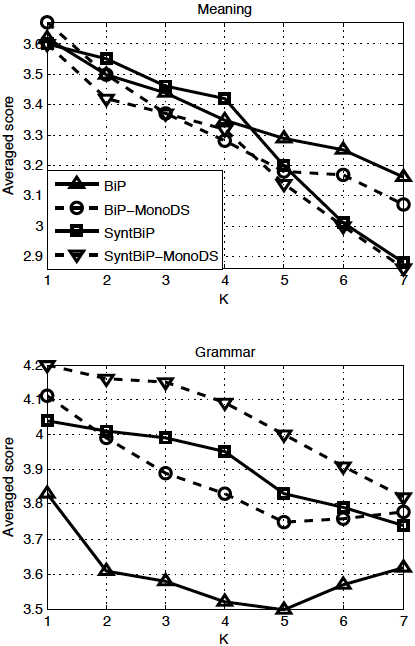
\includegraphics[width=0.78\linewidth]{meanTopK_vertical_LW2_MS8_2} %[width=\linewidth]
\end{center}
\caption{\small Averaged scores in the top K paraphrase candidates as a function of K for different re-ranking metrics. All methods performs similarly in meaning preservation, but SyntBiP-MonoDS outperforms other scoring methods in grammaticality, as shown in the bottom graph.}
\label{fig_meanTopK}
\end{figure}

%\mnote{correlation between human judgment scores and LSH binning} %%%


%%%%%%%%% table for threshold analysis with averaged meaning and grammar scores
% for negative logarithmic BiP probabilities, see bottom of this doc
\begin{table}%[t!] % original version with separate tables and for LSH with support are at the bottom of this doc
\begin{center}
\begin{tabular}{ccc|ccc}%{|l|l|l|}
\hline \hline
\multicolumn{3}{c|} {\bf \scriptsize BiP Paraphrase Score} & \multicolumn{3}{c} {\bf \scriptsize MonoDS LSH Score} \\
\bf \scriptsize Region & \bf \scriptsize M & \bf \scriptsize G & \bf \scriptsize Region & \bf \scriptsize M & \bf \scriptsize G \\ \hline
{\scriptsize 1.00 $\ge$ x $>$ 0.37 } & {\scriptsize 3.6} & {\scriptsize 3.7} & {\scriptsize 1 $\geq$ x $>$ 0.95} & {\scriptsize 4.0} & {\scriptsize 4.4} \\
{\scriptsize 0.37 $\ge$ x $>$ 0.14} & {\scriptsize 3.6} & {\scriptsize 3.7} & {\scriptsize 0.95 $\geq$ x $>$ 0.9} & {\scriptsize 3.2} & {\scriptsize 4.0} \\
{\scriptsize 0.14 $\ge$ x $>$ 0.05} & {\scriptsize 3.4} & {\scriptsize 3.6} & {\scriptsize 0.9 $\geq$ x $>$ 0.85} & {\scriptsize 3.3} & {\scriptsize 4.0} \\
{\scriptsize 0.05 $\ge$ x $>$ 1.8e-2} & {\scriptsize 3.4} & {\scriptsize 3.6} & {\scriptsize 0.85 $\geq$ x $>$ 0.8} & {\scriptsize 3.3} & {\scriptsize 4.0} \\
{\scriptsize 1.8e-2 $\ge$ x $>$ 6.7e-3} & {\scriptsize 3.4} & {\scriptsize 3.6} & {\scriptsize 0.8 $\geq$ x $>$ 0.7} & {\scriptsize 3.2} & {\scriptsize 3.9} \\
{\scriptsize 6.7e-3 $\ge$ x $>$ 2.5e-3} & {\scriptsize 3.2} & {\scriptsize 3.7} & {\scriptsize 0.7 $\geq$ x $>$ 0.6} & {\scriptsize 3.3} & {\scriptsize 3.8} \\
{\scriptsize 2.5e-3 $\ge$ x $>$ 9.1e-4} & {\scriptsize 3.0} & {\scriptsize 3.6} & {\scriptsize 0.6 $\geq$ x $>$ 0.5} & {\scriptsize 3.1} & {\scriptsize 3.7} \\
{\scriptsize 9.1e-4 $\ge$ x $>$ 3.4e-4} & {\scriptsize 3.0} & {\scriptsize 3.8} & {\scriptsize 0.5 $\geq$ x $>$ 0.4} & {\scriptsize 3.1 } & {\scriptsize 3.6}  \\
{\scriptsize 3.4e-4 $\ge$ x $>$ 1.2e-4} & {\scriptsize 2.6} & {\scriptsize 3.6} & {\scriptsize 0.4 $\geq$ x $>$ 0.3} & {\scriptsize 3.1} & {\scriptsize 3.5} \\
{\scriptsize 1.2e-4 $\ge$ x $>$ 4.5e-5} & {\scriptsize 2.7} & {\scriptsize 3.6} & {\scriptsize 0.3 $\geq$ x $>$ 0.2} & {\scriptsize 2.9} & {\scriptsize 3.4} \\
{\scriptsize x $\ge$ 4.5e-5} & {\scriptsize 2.5} & {\scriptsize 3.7} & {\scriptsize 0.2 $\geq$ x $>$ 0.1} & {\scriptsize 3.0} & {\scriptsize 3.3} \\
&&& {\scriptsize 0.1 $\geq$ x $>$ 0} & {\scriptsize 2.9} & {\scriptsize 3.2} \\
\hline
\end{tabular}
\end{center}
\caption{Averaged human judgment scores as a function of binned paraphrase scores and binned LSH scores. %showing the correlation between human judgment and each method for paraphrases candidates extracted by BiP
MonoDS serves as much better thresholding score for extracting high precision paraphrases.}
\label{table9}
\end{table}
% variables from which values are taken from in eval_paraphrase_judgment_hit_Apr2011.py
% avgHmeaning: all avged meaning scores
% cntAvgHmeaning: support ****


One possible use for the paraphrase scores would be as a cutoff threshold where any paraphrases exceeding that value would be selected. Ideally, this would retain only high precision paraphrases.

To verify whether scores from each method correspond to human judgments for paraphrases extracted by BiP, human evaluation scores are averaged for meaning and grammar within each range of paraphrase score for BiP and approximate cosine distance for MonoDS, as shown in Table \ref{table9}. The BiP paraphrase score bin sizes are linear in logarithmic scale. 
%A small value in negative logarithmic paraphrase score associates with better paraphrase quality as evaluated by BiP.

%To verify whether scores of MonoDS via LSH correspond to human judgments for paraphrases extracted by BiP, human evaluation scores are averaged for meaning and grammar within each range of approximate cosine distance, as shown in Table \ref{table9}. 

Observe that for the BiP paraphrase scores on the left panel, no trend on the averaged grammar scores across all score bins is present. While a mild correlation exists between the averaged meaning scores and the paraphrase scores, the top score region (1$>$ x $\ge$ 0) corresponds to merely an averaged value of 3.58 on a 5-point scale. Therefore, thresholding on paraphrase scores among a set of candidates would not guarantee accurate paraphrases in grammar or meaning.


%%%%%%%%% table for COMBINED threshold analysis with averaged meaning and grammar scores
\begin{table}
\begin{center}
\begin{tabular}{c|ccc}
\hline \hline
{\bf \scriptsize MonoDS LSH }& \multicolumn{3}{|c} {\bf \scriptsize BiP Paraphrase Threshold} \\
{\bf \scriptsize Threshold} & \scriptsize $\ge$ 0.05 & \scriptsize $\ge$ 0.01 & \scriptsize $\ge$ 6.7e-3 \\
\hline
\scriptsize $\ge$ 0.9 & \scriptsize 4.2 / 4.4 & \scriptsize 4.1 / 4.4 & \scriptsize 4.0 / 4.4\\
\scriptsize $\ge$ 0.8 & \scriptsize 4.0 / 4.3 & \scriptsize 3.9 / 4.3 & \scriptsize 3.9 / 4.2\\
\scriptsize $\ge$ 0.7 & \scriptsize 3.9 / 4.1 & \scriptsize  3.8 / 4.2 & \scriptsize 3.8 / 4.1\\
\hline
\end{tabular}
\end{center}
\caption{Thresholding using both the MonoDS and BiP scores further improves the average human judgment of Meaning / Grammar.}
\label{table9b}
\end{table}
%Supprt        0.05     0.01    0.0067
%0.9	  	145      375      390
%0.8	 	285      700      795
%0.7	  	365      915      1095
% variables from which values are taken from in eval_paraphrase_judgment_hit_Apr2011.py
% avgHLmeaning: all avged meaning scores
% cntAvgHLmeaning: support ****




On the right panel, MonoDS LSH scores on paraphrase candidates produced by BiP are uniformly higher in grammar than meaning across all score bins, similar to the correlation results in Table \ref{tbl:table4}. The averaged grammar scores decreases monotonically and proportionally to the change in LSH values. With regard to meaning scores, the averaged values roughly correspond to the decrease of LSH values, implying distributional similarity correlates weakly with human judgment in the meaning preservation of paraphrase. Note that the drop in averaged scores is the largest from the top bin (1$\geq$ x $>$ 0.95) to the second bin (0.95 $\geq$ x $>$ 0.9) is the largest within both meaning and grammar. %For example, in the meaning category, while the score goes from 3.99 in the first bin to 3.17 in the second bin, the rest of the bins hovers around 3.20 in the following 6 bins. A similar trend can be observed in the grammar averaged scores as well. 
\textbf{This suggests that thresholding on top tiered LSH scores can be a good filter for extracting high precision paraphrases.} BiP scores, by comparison, are not as useful for thresholding grammaticality. 
%This confirms the observations by \newcite{Snover2010}.


\subsection{Top K Analysis} %%%

Figure \ref{fig_meanTopK} shows the mean human assigned score within the top K candidates averaged across all phrases. 
%Due to different sizes of paraphrase pool for various phrases, the support of the averaged scores decreases from 500 to 100 as K increases. 
Compared across the two categories, meaning scores have lower range of score and a more uniform trend of decreasing values as K grows.  In grammaticality, BiP clearly underperforms whereas the SyntBiP-MonoDS maintains the best score among all methods over all values of K. In addition, a slow drop-off up until K = 4 in the curve for SyntBiP-MonoDS implies that the quality of paraphrases remains relatively high going from top 1 to top 4 candidates.

%\mnote{on max top K candidates}%%%

%%%%%%%%%%%%% Average of **max** of Top K meaning and grammar for each re-ranking score 
\begin{table}%[t!]
\begin{center}
\begin{tabular}{cccc|cc}
%\begin{tabular}{c|cc p{10mm} cp{10mm}}
\hline \hline & &  \multicolumn{4}{c} {\bf \scriptsize Re-ranking Method} \\
& {\bf \scriptsize K} & {\scriptsize BiP} & {\scriptsize BiP-MonoDS} & {\scriptsize SyntBiP} & {\scriptsize SyntBiP-MonoDS} \\
%\begin{tabular}{ccccp{10mm}cc}
%\hline \hline & & & \multicolumn{4}{c} {\bf \scriptsize Re-ranking Method} \\
%& {\bf \scriptsize K} && {\scriptsize BiP} & {\scriptsize BiP-MonoDS} & {\scriptsize SyntBiP} & {\scriptsize SyntBiP-MonoDS} \\
\hline
\multirow{4}{*}{\bf \scriptsize M} & \multicolumn{1}{|c}{\scriptsize 1} & {\scriptsize 3.62 } & \multicolumn{1}{c|}{\scriptsize 3.67} & {\scriptsize 3.58} & {\scriptsize 3.58}\\
&\multicolumn{1}{|c}{\scriptsize 3} & {\scriptsize 4.13}  & \multicolumn{1}{c|} {\scriptsize 4.07} & {\scriptsize 4.13} & {\scriptsize 4.01}\\
&\multicolumn{1}{|c}{\scriptsize 5} & {\scriptsize 4.26}   & \multicolumn{1}{c|} {\scriptsize 4.19}  & {\scriptsize 4.20}  & {\scriptsize 4.09}\\
&\multicolumn{1}{|c}{\scriptsize 10} & {\scriptsize 4.39}   & \multicolumn{1}{c|} {\scriptsize 4.30} & {\scriptsize 4.25} & {\scriptsize 4.23} \\
\hline
\multirow{4}{*} {\bf \scriptsize G} & \multicolumn{1}{|c} {\scriptsize 1} & {\scriptsize 3.83} & \multicolumn{1}{c|} {\scriptsize 4.11} & {\scriptsize 4.04}  & {\scriptsize 4.23}\\
&\multicolumn{1}{|c}{\scriptsize 3} & {\scriptsize 4.22} & \multicolumn{1}{c|} {\scriptsize 4.45}  & {\scriptsize 4.47} & {\scriptsize 4.54}\\
&\multicolumn{1}{|c}{\scriptsize 5}  & {\scriptsize 4.38} & \multicolumn{1}{c|} {\scriptsize 4.54}& {\scriptsize 4.55}  & {\scriptsize 4.62} \\
&\multicolumn{1}{|c}{\scriptsize 10} & {\scriptsize 4.52} & \multicolumn{1}{c|} {\scriptsize 4.62} & {\scriptsize 4.63} & {\scriptsize 4.67} \\
\hline
\end{tabular}
\end{center}
\caption{Average of the \emph{maximum} human evaluation score from top K candidates for each re-ranking method. Support sizes for BiP- and SyntBiP-based metrics are 500 and 335, respectively. (M = Meaning, G = Grammar)} 
\label{table10} 
\end{table}
% variable avgTopK in code, e.g. avgTopK[kTop]['meaning']['hiero']

%%%%%%%%%%%%%% Average of **max** of Top K meaning and grammar for each re-ranking score 
%\begin{table*}%[t!]
%\begin{center}
%\begin{tabular}{rccccccccc}%{|l|l|l|}
%\hline \hline & & \multicolumn{2}{c} {\footnotesize K = 1} &  \multicolumn{2}{c}{\footnotesize K = 3} &  \multicolumn{2}{c}{\footnotesize K= 5} &  \multicolumn{2}{c}{\footnotesize K = 10} \\
%\bf \scriptsize Re-ranking Method & \bf \scriptsize S & \bf \scriptsize M & \bf \scriptsize G  & \bf \scriptsize M & \bf \scriptsize G & \bf \scriptsize M & \bf \scriptsize G & \bf \scriptsize M & \bf \scriptsize G \\ \hline
%{\scriptsize BiP} & {\scriptsize 500} & {\scriptsize 3.62 } & {\scriptsize 3.83} & {\scriptsize 4.13} & {\scriptsize 4.22}  & {\scriptsize 4.26} & {\scriptsize 4.38} & {\scriptsize 4.39} & {\scriptsize 4.52}  \\
%{\scriptsize BiP-MonoDS} & {\scriptsize 500} & {\scriptsize 3.67} & {\scriptsize 4.11} & {\scriptsize 4.07} & {\scriptsize 4.45}  & {\scriptsize 4.19} & {\scriptsize 4.54} & {\scriptsize 4.30} & {\scriptsize 4.62}  \\
%{\scriptsize SyntBiP}& {\scriptsize 335} & {\scriptsize 3.58} & {\scriptsize 4.04} & {\scriptsize 4.13} & {\scriptsize 4.47}  & {\scriptsize 4.20} & {\scriptsize 4.55} & {\scriptsize 4.25} & {\scriptsize 4.63} \\
%{\scriptsize SyntBiP-MonoDS} & {\scriptsize 335} & {\scriptsize 3.58} & {\scriptsize 4.23} & {\scriptsize 4.01} & {\scriptsize 4.54}  & {\scriptsize 4.09} & {\scriptsize 4.62} & {\scriptsize 4.23} & {\scriptsize 4.67} \\
%\hline
%\end{tabular}
%\end{center}
%\caption{Average of the maximum human evaluation score from top K candidates for each re-ranking method (M = Meaning, G = Grammar,  S = Support) }
%\label{table10} 
%\end{table*}
%% variable avgTopK in code, e.g. avgTopK[kTop]['meaning']['hiero']





% @@ examples of LSH better than BiP @@
%\mnote{example of misalignment: 3 examples} %%%
%- considerable changes    1069038 caused quite    1.0     1.0     21.5    1.0  (m:23)
%- always declared 377087  always been     1.0     1.0     19.0    8.0 (m:20)
%- significantly affected  10321   known   2.0     2.5     20.0    4.0 	(max 20)
%@@ example for which LSH helping out Multilingual Pivoting when misalignment is severe (non-sense paraphrases) (1) cite ccb's ppr and mention well-known fact about aligner quality and direct deterioration propagation in pivoting-based (or any grammar-extraction-based method) paraphrase extraction and (2) *briefly* mention potentially incorporating of LSH and tomb counter in improving misalignments, for example, by counting whether aligned phrases co-occur frequent enough in corpus) @@

\begin{table*}
\begin{center}
\begin{tabular}{llcccccc}%{|l|l|l|}
\hline\hline 
&& \multicolumn{4}{c} {\bf \footnotesize Ranking} \\
% example LSH >> BiP
\bf \scriptsize Phrase & \bf \scriptsize Paraphrase & \bf \scriptsize SentID &\bf \scriptsize Size$_{pool}$ & \bf \scriptsize Meaning & \bf \scriptsize Grammar &\bf \scriptsize BiP & \bf \scriptsize BiP-MonoDS \\ \hline
{\scriptsize \emph{significantly affected}} & {\scriptsize \emph{known}} & {\scriptsize 10321}& {\scriptsize 20}  & {\scriptsize 19} & {\scriptsize 18.5} & {\scriptsize 1} & {\scriptsize 17} \\
{\scriptsize \emph{considerable changes}} & {\scriptsize \emph{caused quite}} & {\scriptsize 1069038} & {\scriptsize 23} & {\scriptsize 23} & {\scriptsize 23} & {\scriptsize 2.5} & {\scriptsize 23} \\
{\scriptsize \emph{always declared}} & {\scriptsize \emph{always been}} & {\scriptsize 377087} & {\scriptsize 20} & {\scriptsize 20} & {\scriptsize 20} & {\scriptsize 2} & {\scriptsize 13} \\
\hline
%{\scriptsize urgently adopt, take swift} & {\scriptsize 10} & {\scriptsize 1} & {\scriptsize 2.5} & {\scriptsize 5.5} & {\scriptsize 1} \\
{\scriptsize \emph{hauled}} & {\scriptsize \emph{delivered}} & {\scriptsize 344042} & {\scriptsize 23} & {\scriptsize 7} & {\scriptsize 5.5} & {\scriptsize 21.5} & {\scriptsize 5.0} \\
{\scriptsize \emph{fiscal burden}} & {\scriptsize \emph{taxes}} & {\scriptsize 918627} & {\scriptsize 18} & {\scriptsize 13.5} & {\scriptsize 18} & {\scriptsize 6} & {\scriptsize 16} \\
{\scriptsize \emph{fiscal burden}} & {\scriptsize \emph{taxes}} & {\scriptsize 272831} & {\scriptsize 18} & {\scriptsize 2} & {\scriptsize 8} & {\scriptsize 6} & {\scriptsize 16} \\
%{\scriptsize \emph{of the size, the size of the}} & {\scriptsize 19} & {\scriptsize 186649} & {\scriptsize 11} & {\scriptsize 17} & {\scriptsize 6} & {\scriptsize 15} \\
{\scriptsize \emph{legalise}} & {\scriptsize \emph{legalize}} & {\scriptsize 1104188} & {\scriptsize 23} & {\scriptsize 1} & {\scriptsize 1} & {\scriptsize 10} & {\scriptsize 1} \\
\hline
% example BiP >> LSH
{\scriptsize \emph{to deal properly with}} & {\scriptsize \emph{address}} & {\scriptsize 1156253} & {\scriptsize 35} & {\scriptsize 4.5} & {\scriptsize 5.5} & {\scriptsize 4} & {\scriptsize 29.5} \\
{\scriptsize \emph{you have just stated}} & {\scriptsize \emph{you have just suggested}} & {\scriptsize 129614} & {\scriptsize 31} & {\scriptsize 13.5} & {\scriptsize 8.5} & {\scriptsize 4} & {\scriptsize 30} \\
%{\scriptsize \emph{attackers, forwards on}} & {\scriptsize 34} & {\scriptsize 526677} & {\scriptsize 7.5} & {\scriptsize 6} & {\scriptsize 1} & {\scriptsize 33} \\
%{\scriptsize \emph{}} & {\scriptsize } & {\scriptsize } & {\scriptsize } & {\scriptsize } & {\scriptsize } & {\scriptsize } \\
\hline
\end{tabular}
\end{center}
\caption{Examples of phrase pair rankings by different re-ranking methods and human judgments in terms of meaning and grammar. Higher rank (smaller numbers) corresponds to more favorable paraphrases by the associated metric. Sentence ID is labeled as SentID}
\label{table11}
\end{table*}

% this paragraph refers to table 11 but moved here for formatting
\mnote{remove max K paragraph and Table \ref{table10} if page limit exceeded}In applications such as question answering or search, the order of answers presented is important because the lower an answer is ranked, the less likely it would be looked at by a user. Based on this intuition, the paraphrase ranking methods are evaluated using the maximum human judgment score among the top K candidates obtained by each method. As shown in Table \ref{table10}, when only the top candidate is considered, the averaged score corresponding to the monolingual re-ranking methods are roughly the same as that to the bilingual methods in meaning, but as K grows, the bilingual methods outperforms the monolingual methods. In terms of grammaticality, scores associated with monolingual re-ranking methods are consistently higher than the bilingual methods but the difference tapers off as K increases. This suggests that when only limited top paraphrase candidates can be evaluated, MonoDS is likely to provide better quality of results.



\section{Detailed Examples}
\mnote{need to make sure final formatting puts Table \ref{table11} to the beginning of Section 6}
\subsection{MonoDS Filters Bad BiP Paraphrases}
The examples in the top panel of Table \ref{table11} illustrates a few disadvantages of the bilingual paraphrase scores and how monolingual re-ranking complements the bilingual methods. Translation models based on bilingual corpora are known to suffer from misalignment of the parallel text \cite{BannardCallisonBurch05}, producing incorrect translations that propagate through in the paraphrase model. This issue is exemplified in the phrase pairs \{\emph{considerable changes, caused quite}\}, \{\emph{always declared, always been}\}, and \{\emph{significantly affected, known}\} listed Table \ref{table11}. The paraphrases are clearly unrelated to the corresponding phrases as evident from the low rankings from human judges. Nonetheless, they were included as candidates likely due to misalignment and were ranked relatively high by BiP metric. For example, \emph{considerable changes} was aligned to \emph{modifie consid{\'e}rablement} correctly. However, due to a combination of loose translations and difficulty in aligning multiple words that are spread out in a sentence, the French phrase was inaccurately matched with \emph{caused quite} by the aligner, inducing a bad paraphrase. Note that in these cases LSH produces the results that agrees with the meaning and grammar rankings.


%\mnote{example of LSH helping grammaticality}
%% of the size     186649  the size of the 9.0     3.0     14.0    5.0 (m:19)
%The phrase pair \{\emph{of the size, the size of the}\} may appear in similar context in the training corpora, therefore a rank of 6 out of 19 was assigned by the bilingual metric. However, the actual context of what follows each of the phrases are different by construct, i.e. a quantitative measure and an object should follow the phrases \emph{of the size} and \emph{the size of the}, respectively. For example, one of the sentences goes as follow:
%
%\hangindent=\parindent{\textit{...which fall victim to harassment , from women and the disabled to foreigners and people of a different faith . this gives us an idea \textbf{of the size} of the problem .}}
%
%As such, the paraphrase was ranked 11 and 17 out of 18 by human judges. The clear difference between neighbor content for each of the phrases helps LSH metric to give a low ranking of 15, demonstrating the cue of neighboring content defined by a phrase can be partially accounted for by distributional similarity.

%\emph{we need to encourage innovation in all possible fields , we need to base our economy on knowledge and education and we need to foster entrepreneurship , irrespective \textbf{of the size} of the companies in question .}

\subsection{Context Matters}
%\mnote{effect by context} %%%
% hauled  344042  delivered       17.0    18.5    2.5     19.0
Occasionally, paraphrases are context-dependent, meaning the relevance of the paraphrase depends on the context in a sentence. Bilingual methods can capture limited context through syntactic constraints if the POS tags of the paraphrases and the sentence are available, while the distributional similarity metric, in its current implementation, is purely based on the pattern of co-occurrence with neighboring context n-grams. As a result, LSH scores should be slightly better at gauging the paraphrases defined by context, as suggested by some examples in Table \ref{table11}. The phrase pair \{\emph{hauled, delivered}\} differ slightly in how they describe the manner that an object is moved. However, in the context of the following sentence, they roughly correspond to the same idea:

\hangindent=\parindent{\textit{countries which do not comply with community legislation should be \textbf{hauled} before the court of justice and i think mrs palacio will do so .}

As a result, out of 23 candidates, human judges ranked \emph{delivered} 7 and 5.5 for meaning and grammar, respectively. The monolingual-based metric also assigns a higher rank to the paraphrase while BiP puts it near the lowest rank.

%\mnote{effect by context} %%%
Another example of context-dependency is the phrase pair \{\emph{fiscal burden, taxes}\}, which could have some foreign translations in common. The original phrase appears in the following sentence:

\hangindent=\parindent{\textit{... so that small and medium-sized enterprises can benefit from research investment and the member states can reduce the \textbf{fiscal burden} consisting of taxes and social contributions .}}

The paraphrase candidate \emph{taxes} is no longer appropriate with the consideration of the context surrounding the original phrase. As such,  \emph{taxes} received rankings of 13.5, 18 and 16 out of 18 for meaning, grammar, and MonoDS, respectively, whereas BiP assigns a 6 to the paraphrase. The same phrase pair but a different sentence, the context induces oppose effects on the paraphrase judgments, where the paraphrase received 2 and 8 in the two categories as shown in Table \ref{table11}:

\hangindent=\parindent{\textit{the economic data for our eu as regards employment and economic growth are not particularly good , and , in addition , the \textbf{fiscal burden} in europe , which is to be borne by the citizen , has reached an all-time high of 46 \% . }

Hence, distributional similarity offers additional advantages over BiP only when paraphrase appears in context that also defines most of the non-zero dimensions of the LSH signature vector.

%\mnote{effect of training MonoDS and BiP with different corpora}
An example to illustrate the effect of using different corpora to train the 2 paraphrase re-ranking models is the phrase pair \{\emph{legalise}, \emph{legalize}\}, as shown in Table \ref{table11}. Meaning, grammar and MonoDS all received top rank out of all paraphrases, whereas BiP assigns the paraphrase a rank of 10 out of 23. Since the bilingual pivoting method was trained with Europarl data, which is dominated by British English, BiP fails to acknowledge the American spelling of the same word. On the other hand, distributional similarity feature vectors were extracted from the n-gram corpus with different variations of English, hence this information was constructively informative for paraphrase ranking. This property can be exploited for adaptation of specific domain of paraphrases selection.


 
\subsection{Limitations of MonoDS Implementation}%"Our MonoDS" in title changes it to 2 lines

%\mnote{Additional of sources of error from LSH} %%%
While the monolingual distributional similarity shows promise as a paraphrase ranking method, there are a number of additional drawbacks associated with the implementation.% through LSH. The process of obtaining counts from the n-gram corpus to construct the distributional feature vector requires traversing through the entire collection of N-grams, which takes a substantial amount of time. A revision of the algorithm to allow parallel processing can possibly alleviate such problem. Another issue is the tradeoff between the size of LSH signature vector and the consistency of approximated phrasal cosine distance over multiple repetitions of LSH extraction. While compactness of LSH features in terms of the the number of bits for each feature vector is desirable for computational speed and storage, it sacrifices the accuracy of the phrasal distributional similarity due the the fact that a smaller vector size translates to a greater dependency of the feature vector on the random seeds in the random projection. 

%\mnote{example of sparsity problem} %%%
The method is currently limited to phrases with up to 4 contiguous words that are present in the N-gram corpus for LSH feature vector extraction. Since cosine similarity is a function of the angle between 2 vectors irrespective of the vector magnitudes, thresholding on low occurrences of higher n-grams in the corpus construction causes larger n-grams to suffer from feature sparsity and be susceptible to noise. A few examples from the experiment demonstrate such scenario. For a phrase \emph{to deal properly with}, a paraphrase candidate \emph{address} receives rankings of 4.5, 5.5 and 4 out of 35 for meaning, grammar and BiP, respectively, it is ranked 29.5 by BiP-MonoDS. The two phrases are expected to have similar neighboring context in regular English usage, but it might be misrepresented by the LSH feature vector due to the lack of occurrences of the 4-gram in the corpus.

%\mnote{example of sparsity problem} %%%
Another example of how data sparsity affects LSH feature vectors is the phrase \emph{you have just stated}. An acceptable paraphrase \emph{you have just suggested} was ranked 13.5, 8.5 and 6.5 out of a total of 31 candidates by meaning, grammar and BiP, respectively, but MonoDS only ranks it at 30. The cosine similarity between the phrases are 0.05, which is very low. However, the only tokens that differentiate the 4-gram phrases, i.e. \{\emph{stated},\emph{suggested}\}, have a similarity score of 0.91. This suggests that even though the additional words in the phrase don't alter the meaning significantly, the feature vectors are misrepresented due to the sparsity of the 4-gram. This also demonstrates a weakness of the current implementation of distributional similarity, namely that context within a phrase is not considered for larger n-grams.

%%%%%%%%%%%%%%%%%%%%%%%%%%%%%%%%%%%%%%%%%%%%%%%%%
\section{Conclusions and Future Work}
We have presented a novel paraphrase ranking metric that assigns a score to paraphrase candidates according to their monolingual distributional similarity to the original phrase. While bilingual pivoting-based paraphrase models provides wide coverage of paraphrase candidates and syntactic constraints on the model confines the structural match, additional contextual similarity information provided by monolingual semantic statistics increases the accuracy of paraphrase ranking within the target language. %Reduction of storage and speed gain for distributional features was achieved by LSH approximation of the feature vectors. 
Through a manual evaluation, it was shown that monolingual distributional score strongly correlates with human assessment of paraphrase quality in terms of grammaticality, yet has minimal effects on meaning preservation of paraphrases.

While we speculated that MonoDS would improve both meaning and grammar scoring
for paraphrases based on the fact that contextual similarity entails information
in those dimensions, we found in the results that only grammaticality was
improved from the monolingual approach. This is likely due to the choice of how
context is represented, which in this case is only single neighboring words. A
consideration for future work to enhance paraphrasal meaning preservation would
be to explore other contextual representations, such as syntactic dependency
parsing \cite{LinACL97}, mutual information between co-occurences of phrases
\newcite{ChurchHanks91}, or increasing number of neighboring words used in
n-gram based representations like ours.

A main direction of future work is to take full advantage of the complementary knowledge of paraphrase selection in both bilingual and monolingual ranking schemes by combining the corresponding confidence measures along with other features such as n-gram length, language model scores, etc. One approach would be to perform minimum error rate training similar to \newcite{ZhaoEtAlACL08} in which linear weights of a feature function for a set of paraphrases candidate are trained iteratively to minimize the phrasal-substitution-based error rate. Instead of phrasal substitution in Zhao's method, quantitative measure of correlation with human judgment can be used as the objective function to be optimized during training. Other techniques such as SVM-rank \cite{Joachims02} should also be investigated for aggregating results from multiple ranked lists. 

%The translation score computed with syntactically constrained bilingual paraphrase model implicitly incorporates context dependency for paraphrases through parsing, whereas monolingual distributional similarity inherently lacks such information. One possible modification to the distributional similarity score would be to include the neighboring context in the LSH signature extraction. For example, the word immediately preceding the original phrase in a sentence can be used as the ``right context" concatenated to right-most 3-gram, or less, of the candidate paraphrase, of which a LSH signature can be computed. Similar procedure on the word following the phrase in the sentence would produce a ``left-context" LSH signature. These additional context-dependent features will likely improve the cosine similarity paraphrase ranking.

% re-write the following paragraph: %%%%%%%%%%%%%%%%%%%%%% ================== < here
%Traditional methods for computing distributional similarity scores such as the induction process utilized by \newcite{PascaDienes05}, requires substantial computational storage for collecting contextual counts for each phrase in a large collection as well as the amount of time for computing the quantitative measure of paraphrases. As a result, scalability of these methods hinders paraphrase extraction on large data sets. In our study, monolingual distributional similarity is implemented via Locality Sensitive Hashing, which represents contextual features signatures in small dimensions allowing linear time computation of approximate cosine distance, and can update signature in an online fashion \cite{Charikar02,VanDurmeLallACL10}. This encourages future effort of extending the proposed method to very large sets of candidate paraphrases, as well as the establishing a large database of paraphrases and the corresponding distributional similarity signatures.

%Other future directions include examining the effect on paraphrases scores from an increased number of pivoting languages in the bilingual paraphrase model, eliminating the limitations imposed by the web-scale n-gram corpus on both the maximum length of phrase tokens and the sparsity of features for higher n-grams, training models with domain-specific corpora to extract distributional similarity signatures tailored for certain applications, and explore the possibility of augmenting the paraphrase extraction procedure to include monolingual features in order to alleviate the problems of misalignment.


%@@ briefly mention applying LSH and tomb counter to reduce paraphrase error due to misalignment ?@@

%@@ combination of difference score through minimum error rate training; should combine non-syntactically constrained model with LSH because hiero style provides larger coverage of candidate paraphrases and LSH can increase confidence in the ones that are more likely to be a good paraphrase, whereas syn-contrained model already throws out large number of candidates @@
%@@ the success from pilot study encourages to move from only small amount of test phrases to a large scale evaluation on mechanical turk; maybe even evaluate effect (on coverage, performance, etc) the number of pivoting languages, which will potentially result in larger number of paraphrase candidates per phrase @@
%@@ Synt-constrainted paraphrasing method by construction incorporate context dependency, whereas the information is absent in the monolingual counterpart, so natural next step would be to include context by taking into account the neighboring words of the phrases; hence would introduce 2 additional context-dependent scores into the larger scale of mTurk evaluation @@
%@@feature sparsity issue due to thresholding in google ngram@@



% ccb nikesh: position indep occurence

\bibliographystyle{acl}
\bibliography{references}

\end{document}


%%% table template

\begin{table}%[t!]
\begin{center}
\begin{tabular}{rcc}%{|l|l|l|}
\hline\hline \bf \footnotesize X & \bf \footnotesize X & \bf \footnotesize X \\ \hline
{\scriptsize } & {\scriptsize } & {\scriptsize } \\
{\scriptsize } & {\scriptsize } & {\scriptsize } \\
{\scriptsize } & {\scriptsize }& {\scriptsize } \\
{\scriptsize } & {\scriptsize } & {\scriptsize } \\
\hline 
{\scriptsize } &  {\scriptsize } & {\scriptsize } \\
{\scriptsize }&  {\scriptsize } & {\scriptsize } \\
{\scriptsize } &  {\scriptsize } & {\scriptsize } \\
{\scriptsize }&  {\scriptsize } & {\scriptsize } \\
\hline
\end{tabular}
\end{center}
\caption{\label{tableX} XX}
\end{table}


%%%%%%%%%%%%%%%% TABLE for evaluation w.r.t. Ngram %%%%%%%%%%%%%%%%%%
\begin{table*}%[t!]
\begin{center}
\begin{tabular}{rcccccccc}%{|l|l|l|}
\hline \hline & \multicolumn{2}{c} {N = 1} &  \multicolumn{2}{c}{N = 2} &  \multicolumn{2}{c}{N = 3} &  \multicolumn{2}{c}{N = 4} \\
\bf \scriptsize Re-ranking Method & \bf \scriptsize M & \bf \scriptsize G  & \bf \scriptsize M & \bf \scriptsize G  & \bf \scriptsize M & \bf \scriptsize G  & \bf \scriptsize M & \bf \scriptsize G  \\ \hline
{\scriptsize Hiero-Hiero} & {\scriptsize 0.18 (120)} & {\scriptsize -0.06 (120)}  & {\scriptsize 0.09 (125)} & {\scriptsize -0.03 (125)}  & {\scriptsize 0.15 (120)} & {\scriptsize 0.15 (117)}  & {\scriptsize 0.14 (110)} & {\scriptsize 0.13 (109)}  \\
{\scriptsize Hiero-LSH} & {\scriptsize 0.03 (125)} & {\scriptsize 0.23 (125)}   & {\scriptsize 0.07 (125)} & {\scriptsize 0.17 (125)}  & {\scriptsize 0.13 (124)} & {\scriptsize 0.29 (121)}  & {\scriptsize 0.33 (119)} & {\scriptsize 0.28 (119)}  \\
{\scriptsize SAMT-SAMT}& {\scriptsize 0.20 (99)}& {\scriptsize 0.00 (97)}  & {\scriptsize 0.26 (74)} & {\scriptsize 0.01 (75)}  & {\scriptsize 0.28 (73)} & {\scriptsize 0.26 (68)}  & {\scriptsize -0.06 (54)} & {\scriptsize 0.08 (52)}  \\
{\scriptsize SAMT-LSH} & {\scriptsize 0.13 (104)} & {\scriptsize 0.21 (102)}  & {\scriptsize 0.17 (84)} & {\scriptsize 0.23 (85)}  & {\scriptsize 0.19 (79)} & {\scriptsize 0.22 (74)}  & {\scriptsize 0.13 (59)} & {\scriptsize 0.21 (57)}  \\ 

%{\scriptsize Hiero-Hiero} & {\scriptsize 0.12} & {\scriptsize 0.03} \\
%{\scriptsize Hiero-LSH} & {\scriptsize 0.12} & {\scriptsize \bf 0.23} \\
%{\scriptsize SAMT-SAMT}& {\scriptsize \bf 0.16}& {\scriptsize 0.06} \\
%{\scriptsize SAMT-LSH} & {\scriptsize 0.13} & {\scriptsize 0.20} \\ 
\hline
\end{tabular}
\end{center}
\caption{\label{tableX} {\bf wont be included in ppr} (M = Meaning, G = Grammar,  = Support) Kendall Tau's rank coefficients for correlation of human judgment, collected from Mechanical Turk experiments, in terms of paraphrase meaning and grammaticality with Hiero-based, SAMT-based, and LSH-based translation scores. Numbers with bolded face are the maximum within that column}
\end{table*}
% variables from which values are taken from in eval_paraphrase_judgment_hit_Apr2011.py
% kTauNgram_all_sorted: all Kendal Tau scores
% cntNgram_all: all counts of sentID (i.e. phrase-sentence pair) used to calculate a particular kTau



%%%%%%%%%%%%%%% table for pphrase size analysis, at LEAST size N %%%%%%%%%%%%%%%

\begin{table*}%[t!]
\begin{center}
\begin{tabular}{rccccccccc}%{|l|l|l|}
\hline \hline \bf \scriptsize Re-ranking & \multicolumn{3}{c} {@3} &  \multicolumn{3}{c}{@6} &  \multicolumn{3}{c}{@10} \\
\bf \scriptsize Method & \bf \scriptsize M & \bf \scriptsize G & \bf \scriptsize S & \bf \scriptsize M & \bf \scriptsize G & \bf \scriptsize S & \bf \scriptsize M & \bf \scriptsize G & \bf \scriptsize S \\ \hline
{\scriptsize Hiero-Hiero} & {\scriptsize 0.12} & {\scriptsize 0.03} & {\scriptsize } & {\scriptsize 0.14} & {\scriptsize 0.01} & {\scriptsize } & {\scriptsize 0.14} & {\scriptsize -0.01} & {\scriptsize } \\
{\scriptsize Hiero-LSH} & {\scriptsize 0.13} & {\scriptsize 0.24} & {\scriptsize } & {\scriptsize 0.11} & {\scriptsize 0.26} & {\scriptsize } & {\scriptsize 0.10} & {\scriptsize 0.23} & {\scriptsize } \\
{\scriptsize SAMT-SAMT} & {\scriptsize 0.17} & {\scriptsize 0.08} & {\scriptsize } & {\scriptsize 0.20} & {\scriptsize 0.08} & {\scriptsize } & {\scriptsize 0.21} & {\scriptsize 0.09} & {\scriptsize } \\
{\scriptsize SAMT-LSH} & {\scriptsize 0.17} & {\scriptsize 0.22} & {\scriptsize } & {\scriptsize 0.20} & {\scriptsize 0.23} & {\scriptsize } & {\scriptsize 0.19} & {\scriptsize 0.22} & {\scriptsize } \\
\hline
\end{tabular}
\end{center}
\caption{\label{tableX} {\bf wont be included in ppr} Kendall Tau's rank coefficients for correlation between human judgment and each re-ranking method as a function of the minimum size of paraphrase candidate pool, where meaning, grammar and support are represented as M, G and S, respectively}
\end{table*}

% variables from which values are taken from in eval_paraphrase_judgment_hit_Apr2011.py
% kTauPPsize_all_sorted: all Kendal Tau scores
% cntPPsize_all: all counts of sentID (i.e. phrase-sentence pair) used to calculate a particular kTau



%%%%%%%%%%%%%%%%% table for pphrase size analysis, at MOST size N %%%%%%%%%%%%%%%%%

\begin{table*}%[t!]
\begin{center}
\begin{tabular}{rcccccccc}%{|l|l|l|}
\hline \hline 
%\bf \scriptsize Re-ranking & \multicolumn{3}{c} {@3} &  \multicolumn{3}{c}{@6} &  \multicolumn{3}{c}{@10} &  \multicolumn{3}{c}{@15} &  \multicolumn{3}{c}{@20} &  \multicolumn{3}{c}{@30} \\
 & \multicolumn{2}{c} {\scriptsize BiP} &  \multicolumn{2}{c}{\scriptsize BiP-MonoDS} &  \multicolumn{2}{c}{\scriptsize SyntBiP} &  \multicolumn{2}{c}{\scriptsize SyntBip-MonoDS} \\
\bf \scriptsize $\leq$ N$_{pool size}$ & \bf \scriptsize M & \bf \scriptsize G & \bf \scriptsize M & \bf \scriptsize G & \bf \scriptsize M & \bf \scriptsize G & \bf \scriptsize M & \bf \scriptsize G \\ \hline
{\scriptsize 3} & {\scriptsize 0.24 (36)} & {\scriptsize 0.30 (33)} & {\scriptsize 0.30 (49)} & {\scriptsize 0.21 (47)} & {\scriptsize 1.0 (5)} & {\scriptsize -0.33 (3)}  & {\scriptsize -1.0 (5)} & {\scriptsize 0.33 (3)} \\
{\scriptsize 6} & {\scriptsize 0.16 (90)} & {\scriptsize 0.27 (86)} & {\scriptsize 0.26 (108)} & {\scriptsize 0.25 (105)} & {\scriptsize 0.03 (26)} & {\scriptsize 0.10 (19)} & {\scriptsize -0.34 (26)} & {\scriptsize -0.09 (19)} \\
{\scriptsize 10} & {\scriptsize 0.16 (150)} & {\scriptsize 0.22 (146)} & {\scriptsize 0.24 (168)} & {\scriptsize 0.27 (165)} & {\scriptsize 0.10 (50)} & {\scriptsize 0.10 (43)} & {\scriptsize -0.04 (50)} & {\scriptsize 0.30 (43)} \\
{\scriptsize 15} & {\scriptsize 0.13 (195)} & {\scriptsize 0.18 (191)} & {\scriptsize 0.21(213)} & {\scriptsize 0.28 (210)} & {\scriptsize 0.08 (75)} & {\scriptsize 0.12 (67)} & {\scriptsize 0.01 (83)} & {\scriptsize 0.25 (74)} \\
{\scriptsize 20} & {\scriptsize 0.12 (280)} & {\scriptsize 0.12 (276)} & {\scriptsize 0.18 (298)} & {\scriptsize 0.26 (295)} & {\scriptsize 0.10 (110)} & {\scriptsize 0.10 (102)} & {\scriptsize 0.17 (131)} & {\scriptsize 0.24 (123)} \\
{\scriptsize 30} & {\scriptsize 0.13 (375)} & {\scriptsize 0.07 (371)} & {\scriptsize 0.16 (393)} & {\scriptsize 0.25 (390)} & {\scriptsize 0.21 (200)} & {\scriptsize 0.10 (192)} & {\scriptsize 0.17 (226)} & {\scriptsize 0.23 (218)} \\

\hline
\end{tabular}
\end{center}
\caption{Kendall Tau's rank coefficients for correlation between human judgment and each re-ranking method as a function of the maximum size of paraphrase candidate pool, where the support is indicated in the bracket; meaning and grammar are represented as M and G, respectively}
\label{table7} 
\end{table*}
% variables from which values are taken from in eval_paraphrase_judgment_hit_Apr2011.py
% kTauPPsize_all_sorted: all Kendal Tau scores
% cntPPsize_all: all counts of sentID (i.e. phrase-sentence pair) used to calculate a particular kTau


%%%%%%%%% table for LSH cutoff analysis (replaced by table of the binning of LSH in the ppr)  %%%%%%%%%%%%%
\begin{table}%[t!]
\begin{center}
\begin{tabular}{rcccc}%{|l|l|l|}
\hline \hline
\bf \scriptsize LSH cutoff & \bf \scriptsize Meaning & \bf \scriptsize Grammar & \bf \scriptsize Support \\ \hline
{\scriptsize $\geq$ 0.9} & {\scriptsize 0.19} & {\scriptsize 0.18} & {\scriptsize }  \\
{\scriptsize $\geq$ 0.8} & {\scriptsize 0.24} & {\scriptsize 0.14} & {\scriptsize }  \\
{\scriptsize $\geq$ 0.7} & {\scriptsize 0.15} & {\scriptsize 0.16} & {\scriptsize }  \\
{\scriptsize $\geq$ 0.6} & {\scriptsize 0.10} & {\scriptsize 0.18} & {\scriptsize }  \\
{\scriptsize $\geq$ 0.5} & {\scriptsize 0.13} & {\scriptsize 0.15} & {\scriptsize }  \\
{\scriptsize $\geq$ 0.4} & {\scriptsize 0.12 } & {\scriptsize 0.16} & {\scriptsize }  \\
{\scriptsize $\geq$ 0.3} & {\scriptsize 0.11} & {\scriptsize 0.16} & {\scriptsize }  \\
{\scriptsize $\geq$ 0.2} & {\scriptsize 0.13} & {\scriptsize 0.19} & {\scriptsize }  \\
{\scriptsize $\geq$ 0.1} & {\scriptsize 0.13} & {\scriptsize 0.21} & {\scriptsize }  \\
\hline
\end{tabular}
\end{center}
\caption{Kendall Tau's rank coefficients for correlation between human judgment and LSH score for both meaning and grammar. LSH cutoff is defined as the LSH score above which elements are included in the rank list for calculating Kendall Tau coefficients}
\label{table8}
\end{table}

% variables from which values are taken from in eval_paraphrase_judgment_hit_Apr2011.py
% kTauLSHCutoff_all_sorted: all Kendal Tau scores
% cntLSHCutoff_all: all counts of sentID (i.e. phrase-sentence pair) used to calculate a particular kTau




%\begin{table}%[t!]
%\begin{center}
%\begin{tabular}{ccc}%{|l|l|l|}
%\hline\hline \bf \footnotesize X & \bf \footnotesize X & \bf \footnotesize X \\ \hline
%{\scriptsize } & {\scriptsize } & {\scriptsize } \\
%{\scriptsize } & {\scriptsize } & {\scriptsize } \\
%{\scriptsize } & {\scriptsize }& {\scriptsize } \\
%{\scriptsize } & {\scriptsize } & {\scriptsize } \\
%\hline 
%{\scriptsize } &  {\scriptsize } & {\scriptsize } \\
%{\scriptsize }&  {\scriptsize } & {\scriptsize } \\
%{\scriptsize } &  {\scriptsize } & {\scriptsize } \\
%{\scriptsize }&  {\scriptsize } & {\scriptsize } \\
%\hline
%\end{tabular}
%\end{center}
%\caption{XX}
%\label{table5} 
%\end{table}



%%%%%%%%%%%%%%%%%%%%%%%%%%%%%%%%%%%%%%%%%%%%%%%%%
\subsection{Paraphrase Examples from Urdu-English Corpus}
\label{sect:results_ur_en}
An example shown in Table~\ref{table1} consists of a list of paraphrases generated for the word  {\em unnecessarily} and the corresponding paraphrase scores from each of the 3 confidence metrics. Only the top 5 candidates are shown for the ease of comparison. Out of the top 5 paraphrases, only two from the original bilingual paraphrase extraction are semantically close to actual phrase and none of them are syntactically correct. With the S-C paraphrase model, only the best paraphrase candidate, {\em needlessly}, carries the close enough meaning to {\em unnecessarily}. 

The lack of semantic correspondence in the bilingual methods is likely due to either polysemy in the foreign translation or word alignment mismatch in the bilingual translation. Such problems are not pronounced in the monolingual-based scores. The four paraphrases with the highest LSH-approximated cosine distance are very similar in meaning to the original phrase. Note that cosine distance ranges from -1 to 1 with 1 corresponding to the best match, so the LSH paraphrase candidates in this example are quantitatively close to the true phrase in terms of distributional similarity.

\begin{table}[h]
\begin{center}
\begin{tabular}{ccc}%{|l|l|l|}
\hline\hline \bf \footnotesize BiP & \bf \footnotesize SyntBiP & \bf \footnotesize MonoDS \\ \hline
{\scriptsize necessary (0.118)} & {\scriptsize needlessly (0.024)} & {\scriptsize needlessly (0.93)} \\
{\scriptsize reason (0.084)} & {\scriptsize only (0.012)} & {\scriptsize groundless (0.85)} \\
{\scriptsize unnecessary (0.074)}& {\scriptsize exactly (0.003)}& {\scriptsize unnecessary (0.79)}\\
{\scriptsize same (0.050)} & {\scriptsize just (0.001)} & {\scriptsize useless (0.79)} \\
{\scriptsize useless (0.037)}& {\scriptsize always (0.001)}& {\scriptsize illegally (0.78)}\\
%{\scriptsize necessary (-2.14)} & {\scriptsize needlessly (-3.75)} & {\scriptsize needlessly (0.93)} \\
%{\scriptsize reason (-2.48)} & {\scriptsize only (-4.41)} & {\scriptsize groundless (0.85)} \\
%{\scriptsize unnecessary (-2.60)}& {\scriptsize exactly (-5.80)}& {\scriptsize unnecessary (0.79)}\\
%{\scriptsize same (-2.99)} & {\scriptsize just (-6.74)} & {\scriptsize useless (0.79)} \\
%{\scriptsize useless (-3.30)}& {\scriptsize always (-6.74)}& {\scriptsize illegally (0.78)}\\
\hline
\end{tabular}
\end{center}
\caption{Paraphrases for {\em unnecessarily} according to the original (Hiero), syntactic-constraint-based (SAMT) translation score and the monolingual similarity score(LSH), ranked by corresponding scores in brackets}
\label{table1}
\end{table}

Table~\ref{table2} shows another example of the extracted paraphrases for the phrase {\em huge amount of}. Although monolingual distributional similarity does not explicitly impose syntactic restrictions, the paraphrase {\em in large numbers} in this example was assigned a low score of 0.098 as compared to other paraphrase candidates with correct syntactic type. Its syntactic structure causes its left and right context in the English corpus to be drastically different from that of the original phrase, resulting in a low LSH score. Note that the S-C paraphrase model returns significantly less candidates, which exemplifies the lack of coverage commonly observed in this paraphrase model as mentioned in (Callison-Burch, 2008.) Therefore, it is important to expand the paraphrases for the monolingual scoring by taking the union of candidates from both kinds of bilingual paraphrase model.


\begin{table}[t!]
\begin{center}
\begin{tabular}{ccc}%{|l|l|l|}
\hline\hline 
\bf \small BiP & \bf \small SyntBiP & \bf \small MonoDS \\ \hline

{\scriptsize large number of, 0.33} & {\scriptsize large number of, 0.38} & {\scriptsize large quantity of, 0.98} \\
{\scriptsize in large numbers, 0.11} & {\scriptsize great number of, 0.09} & {\scriptsize large number of, 0.98} \\
{\scriptsize great number of, 0.08}& {\scriptsize vast number of, 0.06}& {\scriptsize great number of, 0.97}\\
{\scriptsize large numbers of, 0.06} & & {\scriptsize vast number of, 0.94} \\
{\scriptsize vast number of, 0.06}& & {\scriptsize in large numbers, 0.10}\\

%{\scriptsize large number of, 0.333} & {\scriptsize large number of, 0.375} & {\scriptsize large quantity of, 0.98} \\
%{\scriptsize in large numbers, 0.111} & {\scriptsize great number of, 0.093} & {\scriptsize large number of, 0.98} \\
%{\scriptsize great number of, 0.084}& {\scriptsize vast number of, 0.063}& {\scriptsize great number of, 0.97}\\
%{\scriptsize large numbers of, 0.056} & & {\scriptsize vast number of, 0.94} \\
%{\scriptsize vast number of, 0.056}& & {\scriptsize in large numbers, 0.10}\\

%{\scriptsize large number of, -1.10} & {\scriptsize large number of, -0.98} & {\scriptsize large quantity of, 0.98} \\
%{\scriptsize in large numbers, -2.20} & {\scriptsize great number of, -2.37} & {\scriptsize large number of, 0.98} \\
%{\scriptsize great number of, -2.48}& {\scriptsize vast number of, -2.77}& {\scriptsize great number of, 0.97}\\
%{\scriptsize large numbers of, -2.89} & & {\scriptsize vast number of, 0.94} \\
%{\scriptsize vast number of, -2.89}& & {\scriptsize in large numbers, 0.10}\\
\hline
\end{tabular}
\end{center}
\caption{Paraphrases for {\em huge amount of} according to the bilingual pivoting (BiP), syntactic-constrainted bilingual pivoting (SyntBiP) translation score and the monolingual similarity score via LSH (MonoDS), ranked by corresponding scores listed next to each paraphrase}}
\label{table2}
\end{table}

%@@ discuss adv and disadv of each of the scores; LSH complementary to the shortfall of paraphrases extracted by parallel corpus, e.g. multiple meaning of foreign word would result in paraphrases that isn't correct at all @@

%@@ LSH score: computation duration due to distributional counts collection, tradeoff between storage/LSH signature vector size and consistency/accuracy of approximated cosine distance due to random seeds required for random projection algorithm; currently only supports contiguous phrases and phrases of up-to-4-gram; ALSO only limited to phrases seen in the n-gram corpus; 

%@@first time applied to paraphrase reranking as compared to previous approaches of paraphrase-extraction entirely based on monolingual parallel corpus; issue/relationship with thresholding similarity score; issue of feature dimension sparsity of higher-n-gram due to occurrence count thresholding in google ngram @@

%@@ word alignment issue - inherent in paraphrase methods based on pivoting, regardless of ranking scores @@

%@@@ mention amount of paraphrases extracted from ur-en


%%%%%%%%%%%%%%%%%%%%%%%%%%%%%%%%%%%%%%%%%%%%%%%%%
\subsection{Pilot Study Results}
\label{sect:results_pilot}

Table \ref{tbl:table3} shows the Kendall's tau coefficients that quantifies the correlation between paraphrase re-ranking scores and human judgment collected using the Mechanical Turk. The positive values listed indicate that both paraphrase measures agree with human judgment in terms of meaning-preservation (0.28 and 0.19 for monolingual and bilingual, respectively) and grammaticality (0.31 and 0.15.) However, human judgment associates stronger with distributional similarity score with significantly higher coefficient values than bilingual translation score, with a larger difference in the grammaticality category. This implies that statistical semantic information provided through distributional similarity is useful for judging the naturalness of paraphrase perceived by humans and provides additional grammatical information as compared to bilingual pivoting-based re-ranking metrics. This conclusion motivates the next experimental study for exploring the benefits of combining monolingual and multilingual resources in the task of paraphrase extraction.

\begin{table}
\begin{center}
\footnotesize
\begin{tabular}{rcc} 
\hline
\hline
 & {\bf MonoDS} & {\bf BiP}\\
 Meaning &  0.28     &  0.19 \\
 Grammar &  0.31   &  0.15 \\
\end{tabular}
\caption{\small Kendall Tau's rank coefficient, comparing the paraphrase ranking quality of monolingual and bilingual scores, with respect to human judgments, for the pilot study.}
\label{tbl:table3}
\end{center}
\end{table}

\mnote{include table of paraphrase examples for ``study in detail" ?}
%The paraphrase candidates generated and ranked by each of the scores are listed in Table \ref{tbl:pp-candidates}. 

%@@ note: context-aware, take information from Courtney's ppr @@
%@@ setup, evaluation method and purposes, examples, overall results, ..@@

% the following table 
%\begin{table}
%\begin{center}
%\footnotesize
%\begin{tabular}{rcc}
%\hline
%\hline
%{\bf Paraphrase} & {\bf Monlingual} & {\bf Bilingual} \\
% study in detail          &  1.00 &  0.70\\
% scrutinise               &  0.94 &  0.08\\
% carefully examine        &  0.93 &  0.08\\
% keep                     &  0.83 &  0.03\\
% studying more closely    &  0.64 &  0.04\\
% analysing                &  0.61 &  0.06\\
%     study                    &  0.42 &  0.07 \\
%     studied                  &  0.28 &  0.01 \\
%     studied in greater depth &  0.13 &  0.02 \\
%     undertook                &  0.06 &  0.06 \\
%\end{tabular}
%\caption{\small \small Subset of 4-gram-or-less paraphrase candidates for {\em study in detail} with corresponding approximate distributional similarity (Monolingual) and translation model (Bilingual) scores.}
%\label{tbl:pp-candidates}
%\end{center}
%\end{table}





%%%%%%%%%%%%% Average of **mean** of Top K meaning and grammar for each re-ranking score %%%%%%%%%%%%%%%%%%
\begin{table*}%[t!]
\begin{center}
\begin{tabular}{rcccccccccccc}%{|l|l|l|}
\hline \hline & \multicolumn{3}{c} {\scriptsize BiP} &  \multicolumn{3}{c}{\scriptsize BiP-MonoDS} &  \multicolumn{3}{c}{\scriptsize SyntBiP} &  \multicolumn{3}{c}{\scriptsize SyntBip-MonoDS} \\
\bf \scriptsize Top K & \bf \scriptsize M & \bf \scriptsize G & \bf \scriptsize S & \bf \scriptsize M & \bf \scriptsize G & \bf \scriptsize S & \bf \scriptsize M & \bf \scriptsize G & \bf \scriptsize S & \bf \scriptsize M & \bf \scriptsize G & \bf \scriptsize S \\ \hline
{\scriptsize 1} & {\scriptsize 3.62} & {\scriptsize 3.83} & {\scriptsize 500} & {\scriptsize 3.67} & {\scriptsize 4.11} & {\scriptsize 500} & {\scriptsize 3.60} & {\scriptsize 4.04} & {\scriptsize 390} & {\scriptsize 3.60} & {\scriptsize 4.20} & {\scriptsize 390}  \\
{\scriptsize 3} & {\scriptsize 3.50} & {\scriptsize 3.61} & {\scriptsize 465} & {\scriptsize 3.50} & {\scriptsize 3.99} & {\scriptsize 465} & {\scriptsize 3.55} & {\scriptsize 4.01} & {\scriptsize 290} & {\scriptsize 3.42} & {\scriptsize 4.16} & {\scriptsize 290}  \\
{\scriptsize 5} & {\scriptsize 3.44} & {\scriptsize 3.58} & {\scriptsize 425} & {\scriptsize 3.37} & {\scriptsize 3.89} & {\scriptsize 425} & {\scriptsize 3.46} & {\scriptsize 3.99} & {\scriptsize 245} & {\scriptsize 3.37} & {\scriptsize 4.15} & {\scriptsize 245}  \\
{\scriptsize 7} & {\scriptsize 3.35} & {\scriptsize 3.52} & {\scriptsize 385} & {\scriptsize 3.28} & {\scriptsize 3.83} & {\scriptsize 385} & {\scriptsize 3.42} & {\scriptsize 3.95} & {\scriptsize 205} & {\scriptsize 3.32} & {\scriptsize 4.09} & {\scriptsize 205}  \\
{\scriptsize 10} & {\scriptsize 3.29} & {\scriptsize 3.50} & {\scriptsize 360} & {\scriptsize 3.18} & {\scriptsize 3.75} & {\scriptsize 360} & {\scriptsize 3.20} & {\scriptsize 3.83} & {\scriptsize 160} & {\scriptsize 3.14} & {\scriptsize 4.00} & {\scriptsize 160}  \\
{\scriptsize 15} & {\scriptsize 3.25} & {\scriptsize 3.57} & {\scriptsize 305} & {\scriptsize 3.17} & {\scriptsize 3.76} & {\scriptsize 305} & {\scriptsize 3.01} & {\scriptsize 3.79} & {\scriptsize 140} & {\scriptsize 3.00} & {\scriptsize 3.91} & {\scriptsize 140}  \\
{\scriptsize 20} & {\scriptsize 3.16} & {\scriptsize 3.62} & {\scriptsize 210} & {\scriptsize 3.07} & {\scriptsize 3.78} & {\scriptsize 210} & {\scriptsize 2.88} & {\scriptsize 3.74} & {\scriptsize 100} & {\scriptsize 2.86} & {\scriptsize 3.82} & {\scriptsize 100}  \\
%\hline \hline \bf \scriptsize Re-ranking & \multicolumn{3}{c} {K = 1} &  \multicolumn{3}{c}{K = 3} &  \multicolumn{3}{c}{K= 5} &  \multicolumn{3}{c}{K = 7} &  \multicolumn{3}{c}{K = 10} &  \multicolumn{3}{c}{K = 15} &  \multicolumn{3}{c}{K = 20} \\
%\bf \scriptsize Method & \bf \scriptsize M & \bf \scriptsize G  & \bf \scriptsize S & \bf \scriptsize M & \bf \scriptsize G & \bf \scriptsize S & \bf \scriptsize M & \bf \scriptsize G & \bf \scriptsize S & \bf \scriptsize M & \bf \scriptsize G & \bf \scriptsize S & \bf \scriptsize M & \bf \scriptsize G & \bf \scriptsize S & \bf \scriptsize M & \bf \scriptsize G & \bf \scriptsize S & \bf \scriptsize M & \bf \scriptsize G & \bf \scriptsize S \\ \hline
%{\scriptsize BiP} & {\scriptsize 3.62} & {\scriptsize 3.83} & {\scriptsize } & {\scriptsize 3.50}  & {\scriptsize 3.61} & {\scriptsize } & {\scriptsize 3.44} & {\scriptsize 3.58} & {\scriptsize } & {\scriptsize 3.35} & {\scriptsize 3.52} & {\scriptsize } & {\scriptsize 3.29} & {\scriptsize 3.50} & {\scriptsize } & {\scriptsize 3.25} & {\scriptsize 3.57} & {\scriptsize }  & {\scriptsize 3.16} & {\scriptsize 3.62} & {\scriptsize } \\
%{\scriptsize BiP-MonoDS}  & {\scriptsize } & {\scriptsize } & {\scriptsize } & {\scriptsize }  & {\scriptsize } & {\scriptsize } & {\scriptsize } & {\scriptsize } & {\scriptsize } & {\scriptsize } & {\scriptsize } & {\scriptsize } & {\scriptsize } & {\scriptsize } & {\scriptsize } & {\scriptsize } & {\scriptsize } & {\scriptsize } & {\scriptsize } & {\scriptsize } & {\scriptsize }  \\
%{\scriptsize SyntBiP} & {\scriptsize } & {\scriptsize } & {\scriptsize } & {\scriptsize }  & {\scriptsize } & {\scriptsize } & {\scriptsize } & {\scriptsize } & {\scriptsize } & {\scriptsize } & {\scriptsize } & {\scriptsize } & {\scriptsize } & {\scriptsize }  & {\scriptsize } & {\scriptsize } & {\scriptsize } & {\scriptsize } & {\scriptsize } & {\scriptsize } & {\scriptsize }  \\
%{\scriptsize SyntBiP-MonoDS} & {\scriptsize } & {\scriptsize } & {\scriptsize } & {\scriptsize }  & {\scriptsize } & {\scriptsize } & {\scriptsize } & {\scriptsize } & {\scriptsize } & {\scriptsize } & {\scriptsize } & {\scriptsize } & {\scriptsize } & {\scriptsize }  & {\scriptsize } & {\scriptsize } & {\scriptsize } & {\scriptsize } & {\scriptsize } & {\scriptsize } & {\scriptsize }  \\
\hline
\end{tabular}
\end{center}
\caption{\emph{convert into a graph later}Average of the mean human evaluation score from top K candidates for each re-ranking method (M = Meaning, G = Grammar,  S = Support) }
\label{table11}
\end{table*}

% variable avgTopKmean in code, e.g. avgTopKmean[kTop]['meaning']['hiero']


\begin{table}%[t!]
\begin{center}
\begin{tabular}{rcc}%{|l|l|l|}
\hline\hline \bf \footnotesize Re-ranking Method & \bf \footnotesize Meaning & \bf \footnotesize Grammar \\ \hline
{\scriptsize BiP} & {\scriptsize 0.14 (475)} & {\scriptsize 0.04 (471)} \\
{\scriptsize BiP-MonoDS} & {\scriptsize 0.14 (493)} & {\scriptsize \bf 0.24 (490)} \\
{\scriptsize SyntBiP} & {\scriptsize \bf 0.19 (300)}& {\scriptsize 0.08 (292)} \\
{\scriptsize SyntBip-MonoDS} & {\scriptsize 0.15 (326)} & {\scriptsize 0.22 (318)} \\
\hline 
{\scriptsize SyntBiP$_{matched}$} &  {\scriptsize 0.20 (179)} & {\scriptsize 0.15 (175)} \\
{\scriptsize SyntBiP$_{matched}$-MonoDS}&  {\scriptsize 0.17 (190)} & {\scriptsize 0.16 (187)} \\
{\scriptsize SyntBiP*} &  {\scriptsize \bf 0.21 (273)} & {\scriptsize 0.09 (266)} \\
{\scriptsize SyntBiP-MonoDS*}&  {\scriptsize 0.16 (295)} & {\scriptsize \bf 0.22 (288)} \\
\hline
\end{tabular}
\end{center}
\caption{Kendall Tau's rank correlation coefficients between human judgment of meaning and grammaticality for the different paraphrase scoring methods. Bottom panel: SyntBiP$_{matched}$ is the same as SyntBiP except paraphrases must match with the original phrase in syntactic type. SyntBiP* and MonoDS* are the same as before except they share the same phrase support with SyntBiP$_{matched}$. The number of human judgments used to calculate the coefficients are listed in parentheses. These numbers vary because many have tied scores so are excluded from Kendall's tau b.}
%\caption{Kendall Tau's rank coefficients for correlation of human judgment in terms of paraphrase meaning and grammaticality with bilingual pivoting (BiP), syntactically-constrained bilingual pivoting (SyntBiP), and monolingual distributional similarity via LSH (MonoDS) paraphrase scores. Bottom panel: SyntBiP$_{matched}$ is the same as SyntBiP except paraphrases must match with the original phrase in syntactic type. SyntBiP* and MonoDS* are the same as before except they share the same phrase support with SyntBiP$_{matched}$. Size of support is listed in brackets. Numbers with bolded face are the maximum within that column}
\label{tbl:table4} 
\end{table}
% variables from which values are taken from in eval_paraphrase_judgment_hit_Apr2011.py
% kTau_all_sorted: all Kendal Tau scores
% cnt_all: all counts of sentID (i.e. phrase-sentence pair) used to calculate a particular kTau


%%%%%%%%% table for LSH cutoff on average meaning and grammar analysis
\begin{table}%[t!]
\begin{center}
\begin{tabular}{rcccc}%{|l|l|l|} ################################### fill in table with results avgLSHgrammar and avgLSHmeaning
\hline \hline
\bf \scriptsize LSH Region & \bf \scriptsize Meaning & \bf \scriptsize Grammar & \bf \scriptsize Support \\ \hline
%{\scriptsize 1 $\geq$ x $>$ 0.9} & {\scriptsize 3.49} & {\scriptsize 4.17} & {\scriptsize 905}  \\
%{\scriptsize 0.9 $\geq$ x $>$ 0.8} & {\scriptsize 3.27} & {\scriptsize 3.98} & {\scriptsize 830}  \\
{\scriptsize 1 $\geq$ x $>$ 0.95} & {\scriptsize 3.99} & {\scriptsize 4.43} & {\scriptsize 350}  \\
{\scriptsize 0.95 $\geq$ x $>$ 0.9} & {\scriptsize 3.17} & {\scriptsize 4.00} & {\scriptsize 555}  \\
{\scriptsize 0.9 $\geq$ x $>$ 0.85} & {\scriptsize 3.25} & {\scriptsize 3.98} & {\scriptsize 470}  \\
{\scriptsize 0.85 $\geq$ x $>$ 0.8} & {\scriptsize 3.30} & {\scriptsize 3.98} & {\scriptsize 360}  \\
{\scriptsize 0.8 $\geq$ x $>$ 0.7} & {\scriptsize 3.21} & {\scriptsize 3.91} & {\scriptsize 750}  \\
{\scriptsize 0.7 $\geq$ x $>$ 0.6} & {\scriptsize 3.27} & {\scriptsize 3.80} & {\scriptsize 935}  \\
{\scriptsize 0.6 $\geq$ x $>$ 0.5} & {\scriptsize 3.08} & {\scriptsize 3.68} & {\scriptsize 915}  \\
{\scriptsize 0.5 $\geq$ x $>$ 0.4} & {\scriptsize 3.1 } & {\scriptsize 3.57} & {\scriptsize 665}  \\
{\scriptsize 0.4 $\geq$ x $>$ 0.3} & {\scriptsize 3.08} & {\scriptsize 3.54} & {\scriptsize 790}  \\
{\scriptsize 0.3 $\geq$ x $>$ 0.2} & {\scriptsize 2.93} & {\scriptsize 3.35} & {\scriptsize 805}  \\
{\scriptsize 0.2 $\geq$ x $>$ 0.1} & {\scriptsize 2.98} & {\scriptsize 3.30} & {\scriptsize 880}  \\
{\scriptsize 0.1 $\geq$ x $>$ 0} & {\scriptsize 2.89} & {\scriptsize 3.21} & {\scriptsize 760}  \\
\hline
\end{tabular}
\end{center}
\caption{Averaged human judgment scores as a function of binned LSH scores for correlation between human judgment and monolingual distributional similarity via LSH in terms of meaning and grammar.}
\label{table9}
\end{table}
% variables from which values are taken from in eval_paraphrase_judgment_hit_Apr2011.py
% kTauLSHCutoff_all_sorted: all Kendal Tau scores
% cntLSHCutoff_all: all counts of sentID (i.e. phrase-sentence pair) used to calculate a particular kTau


%%%%%%%%% table for LSH cutoff on average meaning and grammar analysis
\begin{table}%[t!] % original version with support is at the bottom of this doc
\begin{center}
\begin{tabular}{rccc}%{|l|l|l|} ################################### fill in table with results avgLSHgrammar and avgLSHmeaning
\hline \hline
\bf \scriptsize LSH Region & \bf \scriptsize Meaning & \bf \scriptsize Grammar \\ \hline
%{\scriptsize 1 $\geq$ x $>$ 0.9} & {\scriptsize 3.49} & {\scriptsize 4.17} & {\scriptsize 905}  \\
%{\scriptsize 0.9 $\geq$ x $>$ 0.8} & {\scriptsize 3.27} & {\scriptsize 3.98} & {\scriptsize 830}  \\
{\scriptsize 1 $\geq$ x $>$ 0.95} & {\scriptsize 3.99} & {\scriptsize 4.43} \\
{\scriptsize 0.95 $\geq$ x $>$ 0.9} & {\scriptsize 3.17} & {\scriptsize 4.00} \\
{\scriptsize 0.9 $\geq$ x $>$ 0.85} & {\scriptsize 3.25} & {\scriptsize 3.98} \\
{\scriptsize 0.85 $\geq$ x $>$ 0.8} & {\scriptsize 3.30} & {\scriptsize 3.98} \\
{\scriptsize 0.8 $\geq$ x $>$ 0.7} & {\scriptsize 3.21} & {\scriptsize 3.91} \\
{\scriptsize 0.7 $\geq$ x $>$ 0.6} & {\scriptsize 3.27} & {\scriptsize 3.80} \\
{\scriptsize 0.6 $\geq$ x $>$ 0.5} & {\scriptsize 3.08} & {\scriptsize 3.68} \\
{\scriptsize 0.5 $\geq$ x $>$ 0.4} & {\scriptsize 3.1 } & {\scriptsize 3.57}  \\
{\scriptsize 0.4 $\geq$ x $>$ 0.3} & {\scriptsize 3.08} & {\scriptsize 3.54} \\
{\scriptsize 0.3 $\geq$ x $>$ 0.2} & {\scriptsize 2.93} & {\scriptsize 3.35} \\
{\scriptsize 0.2 $\geq$ x $>$ 0.1} & {\scriptsize 2.98} & {\scriptsize 3.30} \\
{\scriptsize 0.1 $\geq$ x $>$ 0} & {\scriptsize 2.89} & {\scriptsize 3.21} \\
\hline
\end{tabular}
\end{center}
\caption{Averaged human judgment scores as a function of binned LSH scores, showing the correlation between human judgment and MonoDS via LSH for paraphrases candidates are extracted by BiP.}
\label{table9}
\end{table}
% variables from which values are taken from in eval_paraphrase_judgment_hit_Apr2011.py
% kTauLSHCutoff_all_sorted: all Kendal Tau scores
% cntLSHCutoff_all: all counts of sentID (i.e. phrase-sentence pair) used to calculate a particular kTau

%%%%%%%%% table for neg log paraphrase score cutoff on average meaning and grammar analysis
\begin{table}%[t!] 
\begin{center}
\begin{tabular}{cccc}%{|l|l|l|} ################################### fill in table with results avgLSHgrammar and avgLSHmeaning
\hline \hline
%\bf \scriptsize Paraphrase \\\bf \scriptsize Score Region* & \bf \scriptsize Meaning & \bf \scriptsize Grammar \\ \hline
\bf \scriptsize Paraphrase Score Region* & \bf \scriptsize Meaning & \bf \scriptsize Grammar \\ \hline
{\scriptsize 1 $>$ x $\ge$ 0} & {\scriptsize 3.58} & {\scriptsize 3.71} \\
{\scriptsize 2 $>$ x $\ge$ 1} & {\scriptsize 3.59} & {\scriptsize 3.73} \\
{\scriptsize 3 $>$ x $\ge$ 2} & {\scriptsize 3.42} & {\scriptsize 3.56} \\
{\scriptsize 4 $>$ x $\ge$ 3} & {\scriptsize 3.37} & {\scriptsize 3.60} \\
{\scriptsize 5 $>$ x $\ge$ 4} & {\scriptsize 3.36} & {\scriptsize 3.58} \\
{\scriptsize 6 $>$ x $\ge$ 5} & {\scriptsize 3.22} & {\scriptsize 3.65} \\
{\scriptsize 7 $>$ x $\ge$ 6} & {\scriptsize 2.98} & {\scriptsize 3.62}  \\
{\scriptsize 8 $>$ x $\ge$ 7} & {\scriptsize 2.98} & {\scriptsize 3.77} \\
{\scriptsize 9 $>$ x $\ge$ 8} & {\scriptsize 2.56} & {\scriptsize 3.55} \\
{\scriptsize 10 $>$ x $\ge$ 9} & {\scriptsize 2.65} & {\scriptsize 3.60} \\
{\scriptsize x $\ge$ 10} & {\scriptsize 2.47} & {\scriptsize 3.69} \\
\hline
\end{tabular}
\end{center}
\caption{Averaged human judgment scores as a function of binned negative logarithmic paraphrase scores.}
\label{table17}
\end{table}
% variables from which values are taken from in eval_paraphrase_judgment_hit_Apr2011.py
% avgHmeaning: all avged meaning scores
% cntAvgHmeaning: support ****



%%%%%%%%%%%% hand-selected phrases example with 3 significant digits
\begin{table}%[t!]
\begin{center}
\begin{tabular}{lll}%{|l|l|l|}
\hline\hline 
\multicolumn{3}{c} {\bf \footnotesize \emph{reluctant}}\\ \hline
\multicolumn{1}{l}{\bf \footnotesize MonoDS$_{hand-selected}$} & \multicolumn{1}{l} {\bf \footnotesize BiP} \\ \hline
{\scriptsize \emph{*willing} (0.992)} & {\scriptsize \emph{not} (0.558)} & {\scriptsize } \\
{\scriptsize \emph{loath} (0.983)} & {\scriptsize \emph{unwilling} (0.041)} & {\scriptsize } \\
{\scriptsize \emph{*eager} (0.98)}& {\scriptsize \emph{reluctance} (0.031)}& {\scriptsize } \\
{\scriptsize \emph{somewhat reluctant} (0.98)} & {\scriptsize \emph{reticent} (0.025)} \\
{\scriptsize \emph{unable} (0.976)} &  {\scriptsize \emph{hesitant} (0.016)} & {\scriptsize } \\
{\scriptsize \emph{denied access} (0.976)}&  {\scriptsize \emph{reticent about} (0.014)} & {\scriptsize } \\
{\scriptsize \emph{disinclined} (0.976)} &  {\scriptsize \emph{reservations} (0.011)} & {\scriptsize } \\
{\scriptsize \emph{very unwilling} (0.974)}&  {\scriptsize \emph{reticence} (0.010)} & {\scriptsize } \\
{\scriptsize \emph{conducive} (0.973)}&  {\scriptsize \emph{hesitate} (0.009)} & {\scriptsize } \\
{\scriptsize \emph{linked} (0.973)}&  {\scriptsize \emph{are reluctant} (0.009)} & {\scriptsize } \\
\hline
\end{tabular}
\end{center}
\caption{Ordered re-ranked paraphrase candidates for the phrase \emph{reluctant} according to monolingual distributional similarity (MonoDS$_{hand-selected}$) and bilingual pivoting paraphrase (BiP) method. Two hand-selected phrases are labeled with asterisks.}
\label{table6} 
\end{table}



%%%%%%%%% table for threshold analysis with averaged meaning and grammar scores
% BiP scores in this table are neg logarithmic probs
\begin{table}%[t!] % original version with separate tables and for LSH with support are at the bottom of this doc
\begin{center}
\begin{tabular}{ccc|ccc}%{|l|l|l|} ################################### fill in table with results avgLSHgrammar and avgLSHmeaning
\hline \hline
\multicolumn{3}{c|} {\bf \scriptsize BiP Paraphrase Score} & \multicolumn{3}{c} {\bf \scriptsize MonoDS LSH Score} \\
\bf \scriptsize Region & \bf \scriptsize M & \bf \scriptsize G & \bf \scriptsize Region & \bf \scriptsize M & \bf \scriptsize G \\ \hline
{\scriptsize 1 $>$ x $\ge$ 0} & {\scriptsize 3.58} & {\scriptsize 3.71} & {\scriptsize 1 $\geq$ x $>$ 0.95} & {\scriptsize 3.99} & {\scriptsize 4.43} \\
{\scriptsize 2 $>$ x $\ge$ 1} & {\scriptsize 3.59} & {\scriptsize 3.73} & {\scriptsize 0.95 $\geq$ x $>$ 0.9} & {\scriptsize 3.17} & {\scriptsize 4.00} \\
{\scriptsize 3 $>$ x $\ge$ 2} & {\scriptsize 3.42} & {\scriptsize 3.56} & {\scriptsize 0.9 $\geq$ x $>$ 0.85} & {\scriptsize 3.25} & {\scriptsize 3.98} \\
{\scriptsize 4 $>$ x $\ge$ 3} & {\scriptsize 3.37} & {\scriptsize 3.60} & {\scriptsize 0.85 $\geq$ x $>$ 0.8} & {\scriptsize 3.30} & {\scriptsize 3.98} \\
{\scriptsize 5 $>$ x $\ge$ 4} & {\scriptsize 3.36} & {\scriptsize 3.58} & {\scriptsize 0.8 $\geq$ x $>$ 0.7} & {\scriptsize 3.21} & {\scriptsize 3.91} \\
{\scriptsize 6 $>$ x $\ge$ 5} & {\scriptsize 3.22} & {\scriptsize 3.65} & {\scriptsize 0.7 $\geq$ x $>$ 0.6} & {\scriptsize 3.27} & {\scriptsize 3.80} \\
{\scriptsize 7 $>$ x $\ge$ 6} & {\scriptsize 2.98} & {\scriptsize 3.62} & {\scriptsize 0.6 $\geq$ x $>$ 0.5} & {\scriptsize 3.08} & {\scriptsize 3.68} \\
{\scriptsize 8 $>$ x $\ge$ 7} & {\scriptsize 2.98} & {\scriptsize 3.77} & {\scriptsize 0.5 $\geq$ x $>$ 0.4} & {\scriptsize 3.1 } & {\scriptsize 3.57}  \\
{\scriptsize 9 $>$ x $\ge$ 8} & {\scriptsize 2.56} & {\scriptsize 3.55} & {\scriptsize 0.4 $\geq$ x $>$ 0.3} & {\scriptsize 3.08} & {\scriptsize 3.54} \\
{\scriptsize 10 $>$ x $\ge$ 9} & {\scriptsize 2.65} & {\scriptsize 3.60} & {\scriptsize 0.3 $\geq$ x $>$ 0.2} & {\scriptsize 2.93} & {\scriptsize 3.35} \\
{\scriptsize x $\ge$ 10} & {\scriptsize 2.47} & {\scriptsize 3.69} & {\scriptsize 0.2 $\geq$ x $>$ 0.1} & {\scriptsize 2.98} & {\scriptsize 3.30} \\
&&& {\scriptsize 0.1 $\geq$ x $>$ 0} & {\scriptsize 2.89} & {\scriptsize 3.21} \\
\hline
\end{tabular}
\end{center}
\caption{Averaged human judgment scores as a function of binned \emph{negative logarithmic} paraphrase scores and binned LSH scores, showing the correlation between human judgment and each method for paraphrases candidates extracted by BiP}
\label{table9}
\end{table}
% variables from which values are taken from in eval_paraphrase_judgment_hit_Apr2011.py
% avgHmeaning: all avged meaning scores
% cntAvgHmeaning: support ****




%%%%%%%%%%%%%%%%%%%%
%% Text removed by Chris for space
%%%%%%%%%%%%%%%%%%%%

%%%%%%%%%%%%%%%%%%%%%%%%%%%%%%%%%%%%%%%%%%%%%%%%%
\subsection{Data}

In the preliminary study, a bilingual paraphrase model was trained using the parallel corpus between Urdu and English from NIST 2009. This data set, which was collected from newswire and weblogs, consists of roughly 1.7 million words and 200K sentences in each language. The word alignments in this parallel corpus were generated with the Berkeley aligner and the English dataset was parsed using Stanford parser \cite{KleinManning03}. %\newcite{VanDurmeLallNIPS09}%VanDurmeLallACL10} \cite{}

For the experimental study in which human judgment was collected from the Mechanical Turk, the French-English parallel text from the Europarl corpus \cite{Koehn05} was used to train the paraphrase model. The parallel corpus was extracted from proceedings of the European parliament with a total of over 1 million sentences and close to 100 million words in the English text. The rest of grammar extraction preprocessing follows the same procedure for the Urdu-English data. This bilingual corpus is a much larger data set and therefore is expected to provide larger coverage and more reasonable paraphrases.
%%%%%%%%%%%%%%%%%%%%%%%%%%%%%%%%%%%%%%%%%%%%%%%%%

While the training data for the bilingual paraphrase models and the testing data for human evaluation come from the Europarl corpus in which the English structure follows the European parliament proceedings, the data for monolingual distributional similarity feature extractions comes from web-scale n-gram collection consisting of English text from diverse sources. As a result, language statistics from different data are involved in paraphrase selection based on bilingual pivoting followed by monolingual distributional similarity re-ranking.

%%%%%%%%%%%%%%%%%%%%%%%%%%%%%%%%%%%%%%%%%%%%%%%%%

%%%%%%%%%%%%%%%%%%%%%%%%%%%%%%%%%%%%%%%%%%%%%%%%%
\subsection{Preliminary study on Urdu-English data}
\label{sect:results_ur_en}

A small preliminary study of the paraphrasing metrics were performed prior to the experimental work with French-English corpora. Due to the significantly smaller corpus size as compared to the one used in \newcite{CallisonBurch08}, the translation and paraphrase candidates presented here are expected of lesser quality. Nonetheless, the results in this demonstrates the flexibility of the choice of foreign language used in the bilingual pivoting paraphrase extraction.

\begin{table}[h]
\begin{center}
\begin{tabular}{ccc}%{|l|l|l|}
\hline\hline \bf \scriptsize BiP & \bf \scriptsize SyntBiP & \bf \scriptsize MonoDS \\ \hline
{\scriptsize necessary (0.118)} & {\scriptsize needlessly (0.024)} & {\scriptsize needlessly (0.93)} \\
{\scriptsize reason (0.084)} & {\scriptsize only (0.012)} & {\scriptsize groundless (0.85)} \\
{\scriptsize unnecessary (0.074)}& {\scriptsize exactly (0.003)}& {\scriptsize unnecessary (0.79)}\\
{\scriptsize same (0.050)} & {\scriptsize just (0.001)} & {\scriptsize useless (0.79)} \\
{\scriptsize useless (0.037)}& {\scriptsize always (0.001)}& {\scriptsize illegally (0.78)}\\
\hline
\end{tabular}
\end{center}
\caption{Paraphrases for {\em unnecessarily} according to the bilingual pivoting (BiP), syntactic-constrained bilingual pivoting (SyntBiP) and the monolingual distributional similarity (MonoDS) scores, ranked within each column by the scores in brackets}
\label{table1}
\end{table}

An example shown in Table~\ref{table1} consists of a list of top 5 paraphrases generated for the word  {\em unnecessarily} and the corresponding paraphrase scores from each of the 3 confidence metrics. Only {\em unnecessary} and {\em useless} from the original bilingual paraphrase extraction are semantically close to actual phrase but are different syntactically; whereas for SyntBiP, only the best paraphrase candidate, {\em needlessly}, shares close enough meaning with {\em unnecessarily}. 
The lack of semantic correspondence observed in the bilingual methods is likely due to either polysemy in the foreign translation or word alignment mismatch in the bilingual translation. Such problems are not pronounced in the monolingual-based scores. The top LSH scores are close to the maximum Kendall's tau value of 1, indicating that the corresponding paraphrases, such as {\em needlessly}, are quantitatively similar to the true phrase in terms of distributional similarity.


%%%%%%%%%%%%%%%%%%%%%%%%%%%%%%%%%%%%%%%%%%%%%%%%%
\section{Experimental Results}
\label{sect:results_fr_en}

Prior to performing analysis on the data collected from the experiment, preprocessing was performed for data quality control and for correct Kendall's tau calculation. A HIT is rejected if a turker fails on the control questions embedded in the HIT or if more than a pre-defined number of entries are left empty. Ranked lists produced by human judgment for a particular phrase would be tossed out if rankings are equal across all paraphrase candidates. Hence, Kendall's tau coefficients are calculated from various sizes of support, which are indicated along with the results. A total of 100 phrases and 5 sentence per phrase are selected for the experiment, resulting in a maximum support size of 500 for Kendall's tau coefficient calculation.
%%%%%%%%%%%%%%%%%%%%%%%%%%%%%%%%%%%%%%%%%%%%%%%%%

\mnote{BiP: Meaning $>$ Grammar; MonoDS: Grammar $>$ Meaning in both panels} %%%
The characteristics of each re-ranking method can be observed by comparing the coefficients within each row, which corresponds to the correlation between a particular re-ranking method to each of the meaning and grammar scores. In all of the bilingual pivoting approaches, Kendall's tau is higher in meaning preservation than grammaticality. For instance, SyntBiP has a Kendall's tau of 0.19 in meaning, 0.11 higher than that in grammaticality. Contrastingly, distributional similarity metrics correlates more with the grammaticality, except for the case of matched syntactic type, with BiP-MonoDS achieving a coefficient of 0.24 in the grammaticality but only a 0.14 in meaning. Bilingual pivoting without additional constraints is known to perform better in paraphrase extraction in meaning perservation than grammaticality \cite{BannardCallisonBurch05}, whereas with the distributional similarity groups phrases into syntactic classes with less emphasis on the similarity of their actual meaning.The orthogonal advantages of the re-ranking methods will be exploited to construct a more fitting paraphrase re-ranking metric.


%%%%%%%%%%%%%%%%%%%%%%%%%%%%%%%%%%%%%%%%%%%%%%%%%


It should not be too surprising that most of the re-ranking metric correlates less with meaning than grammar judgment because grammaticality is fairly rigidly defined whereas meaning is a subjective measure that varies among individuals and depending on sentence context. As such, human judgement scores on meaning are subjected to more noise and inconsistency, which indirectly contribute to lower Kendall's tau coefficients.

% not related to table7
A similar analysis was performed by breaking up phrases into n-gram categories and the result, which is not included here, was similar to the overall case where re-ranking scores based on bilingual pivoting have higher correlation in meaning and lower in grammar than those based on distributional similarity.


%%%%%%%%%%%%%%%%%%%%%%%%%%%%%%%%%%%%%%%%%%%%%%%%%%


%%%%%%%%% table for pphrase size analysis, at MOST size N
\begin{table}%[t!]
\begin{center}
\begin{tabular}{rcccc}%{|l|l|l|}
\hline \hline 
%\bf \scriptsize Re-ranking & \multicolumn{3}{c} {@3} &  \multicolumn{3}{c}{@6} &  \multicolumn{3}{c}{@10} &  \multicolumn{3}{c}{@15} &  \multicolumn{3}{c}{@20} &  \multicolumn{3}{c}{@30} \\
 & \multicolumn{2}{c} {\scriptsize BiP} &  \multicolumn{2}{c}{\scriptsize BiP-MonoDS} \\
\bf \scriptsize $\leq$ N$_{pool}$ & \bf \scriptsize M & \bf \scriptsize G & \bf \scriptsize M & \bf \scriptsize G \\ \hline
{\scriptsize 3} & {\scriptsize 0.24 (36)} & {\scriptsize 0.30 (33)} & {\scriptsize 0.30 (49)} & {\scriptsize 0.21 (47)} \\
{\scriptsize 6} & {\scriptsize 0.16 (90)} & {\scriptsize 0.27 (86)} & {\scriptsize 0.26 (108)} & {\scriptsize 0.25 (105)} \\
{\scriptsize 10} & {\scriptsize 0.16 (150)} & {\scriptsize 0.22 (146)} & {\scriptsize 0.24 (168)} & {\scriptsize 0.27 (165)} \\
{\scriptsize 15} & {\scriptsize 0.13 (195)} & {\scriptsize 0.18 (191)} & {\scriptsize 0.21(213)} & {\scriptsize 0.28 (210)} \\
{\scriptsize 20} & {\scriptsize 0.12 (280)} & {\scriptsize 0.12 (276)} & {\scriptsize 0.18 (298)} & {\scriptsize 0.26 (295)} \\
{\scriptsize 30} & {\scriptsize 0.13 (375)} & {\scriptsize 0.07 (371)} & {\scriptsize 0.16 (393)} & {\scriptsize 0.25 (390)} \\

\hline
\end{tabular}
\end{center}
\caption{Kendall's tau rank coefficients for correlation between human judgment and 2 re-ranking methods as a function of the maximum size of paraphrase candidate pool. Support is indicated in the bracket; meaning and grammar are represented as M and G, respectively}
\label{table7} 
\end{table}
% variables from which values are taken from in eval_paraphrase_judgment_hit_Apr2011.py
% kTauPPsize_all_sorted: all Kendal Tau scores
% cntPPsize_all: all counts of sentID (i.e. phrase-sentence pair) used to calculate a particular kTau


\mnote{effect of paraphrase candidate pool sizes} %%%
The effects from the paraphrase candidate pool sizes are illustrated in Table \ref{table7}. Both ranking metrics decrease gradually in correlation with human judgment in meaning as the number of available paraphrases grows. The same relationship occurs for BiP in the grammaticality but the Kendal's tau stays roughly the same, which implies that even at large numbers of paraphrase candidates, distributional similarity can serve as a metric   close to human judgment in ordering grammaticality.


%%%%%%%%%%%%%%%%%%%%%%%%%%%%%%
%%%%%%%%%%%%%%%%%%%%%%%%%%%%%%


%%%%%%%%%%%%% Average of **max** of Top K meaning and grammar for each re-ranking score 
\begin{table}%[t!]
\begin{center}
\begin{tabular}{ccccp{10mm}cc}
\hline \hline & & & \multicolumn{4}{c} {\bf \scriptsize Re-ranking Method} \\
& {\bf \scriptsize K} && {\scriptsize BiP} & {\scriptsize BiP-MonoDS} & {\scriptsize SyntBiP} & {\scriptsize SyntBiP-MonoDS} \\
\hline
\multirow{4}{*}{\scriptsize 1} & & \bf \scriptsize  M & {\scriptsize 3.62 } & {\scriptsize 3.67} & {\scriptsize 3.58} & {\scriptsize 3.58}\\
& {\scriptsize 1} & \bf \scriptsize G  & {\scriptsize 3.83} & {\scriptsize 4.11} & {\scriptsize 4.04}  & {\scriptsize 4.23}\\
&{\scriptsize 3} & \bf \scriptsize M & {\scriptsize 4.13}  & {\scriptsize 4.07} & {\scriptsize 4.13} & {\scriptsize 4.01}\\
&{\scriptsize 3} & \bf \scriptsize G & {\scriptsize 4.22} & {\scriptsize 4.45}  & {\scriptsize 4.47} & {\scriptsize 4.54}\\
\hline
\multirow{4}{*}{\scriptsize 5} & & \bf \scriptsize M & {\scriptsize 4.26}   & {\scriptsize 4.19}  & {\scriptsize 4.20}  & {\scriptsize 4.09}\\
&{\scriptsize 5} & \bf \scriptsize G   & {\scriptsize 4.38} & {\scriptsize 4.54}& {\scriptsize 4.55}  & {\scriptsize 4.62} \\
&{\scriptsize 10} & \bf \scriptsize M & {\scriptsize 4.39}   & {\scriptsize 4.30} & {\scriptsize 4.25} & {\scriptsize 4.23} \\
&{\scriptsize 10} & \bf \scriptsize G & {\scriptsize 4.52} & {\scriptsize 4.62} & {\scriptsize 4.63} & {\scriptsize 4.67} \\
\hline
\end{tabular}
\end{center}
\caption{Average of the maximum human evaluation score from top K candidates for each re-ranking method, where the size of support for BiP and BiP-MonoDS is 500, for SyntBiP and SyntBiP-MonoDS is 335. (M = Meaning, G = Grammar) }
\label{table14} 
\end{table}
% variable avgTopK in code, e.g. avgTopK[kTop]['meaning']['hiero']




%%%%%%%%%%%%%%%%%%%%%%%%%%%%%%
%%%%%%%%%%%%%%%%%%%%%%%%%%%%%%




In this paper we:
\begin{itemize}
\item Show that monolingual cosine similarity calculated on large volumes texts ranks bilingually extracted paraphrases better than the paraphrase probability originally defined by \newcite{BannardCallisonBurch05} in terms of grammaticality.
\item \mnote{We should probably scrap this bullet} Demonstrate that monolingual distributional similarity can be implemented by Locality Sensitive Hashing, a computationally efficient approximation algorithm that has recently been extended to online signature generation \cite{Charikar02,VanDurmeLallACL10} 
\item Investigate and identify the strength and weaknesses of scoring paraphrases using monolingual distributional similarity versus the bilingually calculated paraphrase probability, and suggest was of combining the different scores in the future.
\end{itemize}





%%%%%%%%%%%%%%%%%%%%%%%%%%%%%%
%%%%%%%%%%%%%%%%%%%%%%%%%%%%%%


{\bf Effects of human judgment quality on gold standard}
%@@ human judgment isn't entirely correct, depending on turker experience with task, with English; context of sentences, length, etc @@
Despite the ease of setup and the economical benefits, subjective evaluation using Mechanical Turk are susceptible to multiple sources of error, causing substantial amount of noise in the collected data. First of all, turker's proficiency in English in terms of either age or language nativeness, would affect how the contextual clues are interpreted, which consequently influence the judgment of the paraphrases. Moreover, the experience in working on HITs and the consistency among, as well as within, turkers would also have an influence in the result quality. 

An example of noisy human judgment is one of the paraphrases generated for the phrase \emph{attackers}. Paraphrase candidate \emph{forwards on} was ranked 7\.5, 6, and 1 out of 34 candidates for meaning, grammar and bilingual-pivoting paraphrase score, respectively, whereas monolingual-based method ranks it at 33. This paraphrase is apparently incorrect but was likely to be generated from misalignment in grammar extraction stage. The actual human scores shows that, with respect to a full score of 5, "forwards on" received 2 and 4 for meaning and 4 and 5 for grammar. These scores do not correlate to the actual paraphrase quality and demonstrates one of the potential noises by human in the data for that influence quality of paraphrase gold standard.
